\documentclass[journal=langd5,manuscript=article]{achemso}
%DIF LATEXDIFF DIFFERENCE FILE
%DIF DEL optimizing01.tex   Sat Feb 16 07:06:35 2019
%DIF ADD optimizing02.tex   Sat Feb 23 11:44:54 2019

\usepackage[version=4]{mhchem} % Formula subscripts using \ce{}
\usepackage{chemfig}
\setatomsep{1.5em}
\newcommand\setpolymerdelim[2]{\def\delimleft{#1}\def\delimright{#2}}

\def\makebraces(#1,#2)#3#4#5{%
  \edef\delimhalfdim{\the\dimexpr(#1+#2)/2}%
  \edef\delimvshift{\the\dimexpr(#1-#2)/2}%
  \chemmove{
    \node[at=(#4),yshift=(\delimvshift)]
      {$
       \left\delimleft
         \vrule height\delimhalfdim depth\delimhalfdim width0pt
       \right.
      $};
    \node[at=(#5),yshift=(\delimvshift)]
      {$
        \left.
          \vrule height\delimhalfdim depth\delimhalfdim width0pt
        \right\delimright_{\rlap{#3}}
      $};
  }%
}

\usepackage[separate-uncertainty=true,multi-part-units=single]{siunitx}

\usepackage{xcolor}
\graphicspath{{figures/}}

\newcommand{\avg}[1]{\left< #1 \right>}
\newcommand{\FIXME}[1]{{\color{red} #1}}

%%%%%%%%%%%%%%%%%%%%%%%%%%%%%%%%%%%%%%%%%%%%%%%%%%%%%%%%%%%%%%%%%%%%%
%% If issues arise when submitting your manuscript, you may want to
%% un-comment the next line.  This provides information on the
%% version of every file you have used.
%%%%%%%%%%%%%%%%%%%%%%%%%%%%%%%%%%%%%%%%%%%%%%%%%%%%%%%%%%%%%%%%%%%%%
%%\listfiles

\author{Christine Middleton}
\author{Mark D. Hannel}
\author{Andrew D. Hollingsworth}
\author{David J. Pine}
\author{David G. Grier}
\email{david.grier@nyu.edu}
\affiliation[NYU]
{Department of Physics and Center for Soft Matter Research,
New York University, New York, NY 10003}

\title[Optimizing colloidal synthesis]
  {Optimizing the synthesis of monodisperse colloidal spheres
  using holographic particle characterization}

%%%%%%%%%%%%%%%%%%%%%%%%%%%%%%%%%%%%%%%%%%%%%%%%%%%%%%%%%%%%%%%%%%%%%
%% Some journals require a list of abbreviations or keywords to be
%% supplied. These should be set up here, and will be printed after
%% the title and author information, if needed.
%%%%%%%%%%%%%%%%%%%%%%%%%%%%%%%%%%%%%%%%%%%%%%%%%%%%%%%%%%%%%%%%%%%%%
\abbreviations{TPM, AIBN, ACHN, KPS, APS, SDS}
\keywords{Holographic video microscopy, particle characterization, colloids}
%DIF PREAMBLE EXTENSION ADDED BY LATEXDIFF
%DIF UNDERLINE PREAMBLE %DIF PREAMBLE
\RequirePackage[normalem]{ulem} %DIF PREAMBLE
\RequirePackage{color}\definecolor{RED}{rgb}{1,0,0}\definecolor{BLUE}{rgb}{0,0,1} %DIF PREAMBLE
\providecommand{\DIFadd}[1]{{\protect\color{blue}\uwave{#1}}} %DIF PREAMBLE
\providecommand{\DIFdel}[1]{{\protect\color{red}\sout{#1}}}                      %DIF PREAMBLE
%DIF SAFE PREAMBLE %DIF PREAMBLE
\providecommand{\DIFaddbegin}{} %DIF PREAMBLE
\providecommand{\DIFaddend}{} %DIF PREAMBLE
\providecommand{\DIFdelbegin}{} %DIF PREAMBLE
\providecommand{\DIFdelend}{} %DIF PREAMBLE
\providecommand{\DIFmodbegin}{} %DIF PREAMBLE
\providecommand{\DIFmodend}{} %DIF PREAMBLE
%DIF FLOATSAFE PREAMBLE %DIF PREAMBLE
\providecommand{\DIFaddFL}[1]{\DIFadd{#1}} %DIF PREAMBLE
\providecommand{\DIFdelFL}[1]{\DIFdel{#1}} %DIF PREAMBLE
\providecommand{\DIFaddbeginFL}{} %DIF PREAMBLE
\providecommand{\DIFaddendFL}{} %DIF PREAMBLE
\providecommand{\DIFdelbeginFL}{} %DIF PREAMBLE
\providecommand{\DIFdelendFL}{} %DIF PREAMBLE
%DIF LISTINGS PREAMBLE %DIF PREAMBLE
\RequirePackage{listings} %DIF PREAMBLE
\RequirePackage{color} %DIF PREAMBLE
\lstdefinelanguage{DIFcode}{ %DIF PREAMBLE
%DIF DIFCODE_UNDERLINE %DIF PREAMBLE
  moredelim=[il][\color{red}\sout]{\%DIF\ <\ }, %DIF PREAMBLE
  moredelim=[il][\color{blue}\uwave]{\%DIF\ >\ } %DIF PREAMBLE
} %DIF PREAMBLE
\lstdefinestyle{DIFverbatimstyle}{ %DIF PREAMBLE
	language=DIFcode, %DIF PREAMBLE
	basicstyle=\ttfamily, %DIF PREAMBLE
	columns=fullflexible, %DIF PREAMBLE
	keepspaces=true %DIF PREAMBLE
} %DIF PREAMBLE
\lstnewenvironment{DIFverbatim}{\lstset{style=DIFverbatimstyle}}{} %DIF PREAMBLE
\lstnewenvironment{DIFverbatim*}{\lstset{style=DIFverbatimstyle,showspaces=true}}{} %DIF PREAMBLE
%DIF END PREAMBLE EXTENSION ADDED BY LATEXDIFF

\begin{document}

%%%%%%%%%%%%%%%%%%%%%%%%%%%%%%%%%%%%%%%%%%%%%%%%%%%%%%%%%%%%%%%%%%%%%
%% The "tocentry" environment can be used to create an entry for the
%% graphical table of contents. It is given here as some journals
%% require that it is printed as part of the abstract page. It will
%% be automatically moved as appropriate.
%%%%%%%%%%%%%%%%%%%%%%%%%%%%%%%%%%%%%%%%%%%%%%%%%%%%%%%%%%%%%%%%%%%%%
\begin{tocentry}
  %DIF <  Some journals require a graphical entry for the Table of Contents.
%DIF <  This should be laid out ``print ready'' so that the sizing of the
%DIF <  text is correct.
\DIFdelbegin %DIFDELCMD < 

%DIFDELCMD < %%%
%DIF <  Inside the \texttt{tocentry} environment, the font used is Helvetica
%DIF <  8\,pt, as required by \emph{Journal of the American Chemical
%DIF <  Society}.
%DIFDELCMD < 

%DIFDELCMD < %%%
%DIF <  The surrounding frame is 9\,cm by 3.5\,cm, which is the maximum
%DIF <  permitted for  \emph{Journal of the American Chemical Society}
%DIF <  graphical table of content entries. The box will not resize if the
%DIF <  content is too big: instead it will overflow the edge of the box.
%DIFDELCMD < 

%DIFDELCMD < %%%
%DIF <  This box and the associated title will always be printed on a
%DIF <  separate page at the end of the document.
  \DIFdelend \centering
 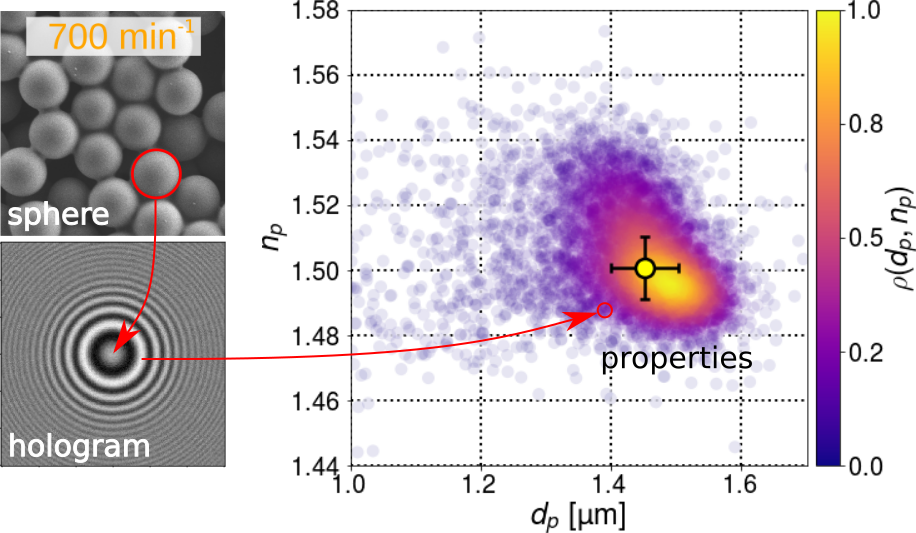
\includegraphics[height=3.5cm]{tocgraphic}
\end{tocentry}

\begin{abstract}
Holographic particle characterization
measures the sizes and compositions of 
individual colloidal particles dispersed in fluid media
and rapidly amasses statistics on the distributions
of these properties, even for complex heterogeneous dispersions.
This information is useful for 
analyzing and optimizing \DIFdelbegin \DIFdel{synthetic protocols }\DIFdelend \DIFaddbegin \DIFadd{protocols for synthesizing
colloidal particles}\DIFaddend .
We illustrate how holographic characterization can guide 
process design through a case study
on a particularly versatile model system
composed of \DIFaddbegin \DIFadd{an aqueous dispersion of }\DIFaddend micrometer-scale
spheres \DIFdelbegin \DIFdel{, which are }\DIFdelend synthesized from the 
organosilane monomer 
3-(trimethoxysilyl)propyl methacrylate
(TPM)\DIFdelbegin \DIFdel{and dispersed in
aqueous media}\DIFdelend .
\end{abstract}

\section{Introduction}
\label{sec:introduction}

Since the serendipitous discovery that emulsion polymerization
can produce colloidal dispersions with very small polydispersity
in size
\cite{backus1949small,gerould1950comments},
techniques for synthesizing
monodisperse colloidal particles have progressed
through trial-and-error experimentation
inspired by principles of chemistry and physics 
and validated \DIFdelbegin \DIFdel{through }\DIFdelend \DIFaddbegin \DIFadd{by }\DIFaddend batteries of particle-characterization
measurements 
\cite{vanderhoff1956some,stober1968controlled,kotera1970colloid,dezelic1970preparation,goodwin1974studies,antl1986preparation}.
How process choices influence the properties of synthetic colloids
typically can be gauged only after
synthesis is complete;
assessing the outcome \DIFdelbegin \DIFdel{typically }\DIFdelend \DIFaddbegin \DIFadd{often }\DIFaddend requires
multiple orthogonal measurement techniques.
Scanning electron microscopy, for example, is used to measure
solid particles' size distribution and surface texture \cite{yamada85}.
Mercury porosimetry and gas adsorption gauge their porosity
\cite{giesche2006mercury} and surface area \cite{rouquerol1994}. 
Refractometry and light scattering probe their optical properties
\cite{chou54}.
Using such techniques to amass a representative 
set of characterization results
takes time and requires expertise.
Preparing samples for measurement, moreover, often involves
transferring particles out of their native medium,
and so can change their properties.
Correlations among particles' properties are especially
difficult to measure, particularly in heterogeneous
dispersions.

Holographic particle characterization can streamline
the design and optimization of colloidal synthesis processes
by providing particle-resolved assays of samples' size distributions
and compositions rapidly and with minimal sample preparation.
Holographic characterization works equally
well for \DIFaddbegin \DIFadd{fluid }\DIFaddend droplets and solid particles
\DIFaddbegin \DIFadd{\mbox{%DIFAUXCMD
\cite{cheong11,philips2017holographic}}\hspace{0pt}%DIFAUXCMD
}\DIFaddend .
It naturally accommodates heterogeneous
samples \DIFaddbegin \DIFadd{\mbox{%DIFAUXCMD
\cite{lee07a,yevick2014machine}}\hspace{0pt}%DIFAUXCMD
,
}\DIFaddend and reveals correlations between size and composition
\DIFaddbegin \DIFadd{\mbox{%DIFAUXCMD
\cite{cheong11,wang2016fractal}}\hspace{0pt}%DIFAUXCMD
}\DIFaddend .
Extensions to the technique
provide particle-resolved morphology measurements from the same underlying data.
All of this information \DIFdelbegin \DIFdel{about a sample's properties can be acquired }\DIFdelend \DIFaddbegin \DIFadd{can be obtained }\DIFaddend with a
single measurement in about ten minutes, which
expedites systematic assays and can be fast enough to provide feedback
for process control.

To illustrate the use of holographic particle characterization
to guide process design, \DIFdelbegin \DIFdel{this }\DIFdelend \DIFaddbegin \DIFadd{the present }\DIFaddend work
explores the roles of emulsion stoichiometry, initiator choice, and
agitation conditions in the synthesis of monodisperse spheres of
3-(trimethoxysilyl)propyl methacrylate (TPM) \cite{vanderwel17},
a model system with increasingly widespread applications
in soft-matter research \cite{sacanna11,liu16,vanderwel18}.
We apply holographic characterization
to identify factors that influence size selection, polydispersity
and composition and validate the results with conventional particle
characterization techniques.
This study therefore builds on the work of van der Wel, \emph{et al.}
\cite{vanderwel17}, which \DIFdelbegin \DIFdel{relies on }\DIFdelend \DIFaddbegin \DIFadd{introduced the synthesis of TPM colloids
and deployed }\DIFaddend conventional techniques to systematically
characterize the emulsion polymerization protocol\DIFdelbegin \DIFdel{for TPM spheres.
}\DIFdelend \DIFaddbegin \DIFadd{.
Our holographic measurements confirm that a straightforward
tabletop synthesis yields exceptionally monodisperse spheres,
and reproduces the observation \mbox{%DIFAUXCMD
\cite{vanderwel17}
}\hspace{0pt}%DIFAUXCMD
that smaller particles form at higher pH.
Holographic analysis also confirms that increasing
monomer concentration tends to form larger spheres,
but reveals that this enhancement decreases as pH increases.
Holographic particle characterization also reveals that more vigorous
mixing during emulsification yields larger
particles without necessarily increasing polydispersity.
This surprising observation runs counter to the usual trend in
emulsion polymerization processes.
Also surprising is the observation that the
choice of free-radical initiator has no discernable
effect on the final particles' properties, at least not
in the range of particle sizes we considered.
These observations help to make our central point that holographic
characterization provides a rich source of information
for choosing among synthesis options in real time
without requiring special sample preparation.
}\DIFaddend 

\section{Materials and methods}
\label{sec:experimental}

\subsection{Materials}
\label{sec:materials}
The TPM monomer (3-(trimethoxysilyl)propyl methacrylate, \SI{98}{\percent})
used in particle synthesis was purchased from Sigma Aldrich. 
Ammonium hydroxide (\SI{29}{\percent}) in water was added to adjust
the pH of the synthesis environment.
Two water-insoluble initiators, 2,2'-azobis(2-methylpropionitrile) (AIBN)
and 1,1'-azobis(cyclohexanecarbonitrile) (ACHN)
were purchased from Sigma Aldrich.
Two water-soluble initiators, 
ammonium persulfate (APS) and potassium persulfate (KPS),
also were purchased from Sigma Aldrich.
\DIFaddbegin \DIFadd{All reagents were used as delivered.
}\DIFaddend 

\subsection{Emulsion polymerization}
\label{ssec:polymerization}

The protocols analyzed in this work focus on 
the influence of stir rate, pH, emulsion stoichiometry, and 
choice of radical initiation 
on the size, polydispersity, and refractive index of
synthesized particles.
While this list is not exhaustive,
it illustrates choices made in optimizing synthetic protocols and the role
that holographic characterization can play in making successful choices.

The synthesis begins with the formation of an emulsion of monodisperse TPM droplets.
Monomeric TPM is insoluble in water but hydrolyzes into
soluble monomers in the basic environment 
of an aqueous ammonium hydroxide solution ($\text{pH} > \num{9}$):
\begin{equation}
\ce{R-Si (OCH3)3 + 3 H2O
    <=>[\text{cat.}][$\text{pH} > 9$]
    R-Si (OH)3 + 3 CH_3OH} ,
\end{equation}
where
\begin{equation}
\schemestart
    \setpolymerdelim()
    R = \chemfig{
    -[@{op,0.5}]-[:-30]-[:30]-[:-30]O-[:30](=[2]O)-[:-30](=[6])-[:30]-[@{cl,0.25}:-30,,,,draw=none]
    }
    \makebraces(5pt,5pt){}{op}{cl}.
\schemestop
\end{equation}
Hydrolyzed monomers then condense into dimers,
\begin{equation}
\ce{2 R-Si (OH)3
    <=>
    \chemfig{HO-Si(-[2]R)(-[6]OH)-O-Si(-[2]R)(-[6]OH)-OH}
    + H2O},
\end{equation}
and higher-order branched silsesquioxanes\DIFaddbegin \DIFadd{.
These oligomers are }\DIFaddend functionalized
with propyl methacrylate groups \DIFdelbegin \DIFdel{that }\DIFdelend \DIFaddbegin \DIFadd{and so }\DIFaddend are insoluble in water\DIFdelbegin \DIFdel{and
}\DIFdelend \DIFaddbegin \DIFadd{.
They therefore }\DIFaddend coalesce homogeneously into monodisperse droplets\DIFdelbegin \DIFdel{.
These nuclei }\DIFdelend \DIFaddbegin \DIFadd{,
which }\DIFaddend continue to grow in a well-mixed environment until
the hydrolyzed monomer is depleted.
\DIFaddbegin 

\DIFaddend At this point, the droplets still are fluid\DIFaddbegin \DIFadd{,
}\DIFaddend but are largely stable against coarsening
\DIFdelbegin \DIFdel{,
}\DIFdelend because of surface charging \cite{vanderwel17}.
They can be transformed into solid spheres by warming
the emulsion to \SI{80}{\degreeCelsius} and adding 
a heat-activated free radical initiator
to polymerize the methacrylate moieties of
the condensed oligomers.

All samples are prepared in identical \SI{12}{\milli\liter}
glass vials to produce \SI{5}{\milli\liter} of colloidal dispersion.
The vials are sealed to ensure consistent evaporation of ammonia
from run to run.
Identical stir bars are used for all syntheses to ensure consistent
flow properties.
\DIFaddbegin \DIFadd{Each synthesis is repeated at least once, and characterization data
compared to ensure consistent results.
}\DIFaddend 

\subsection{Holographic particle characterization}
\label{sec:holographicparticlecharacterization}

\begin{figure}[!b]
    \centering
    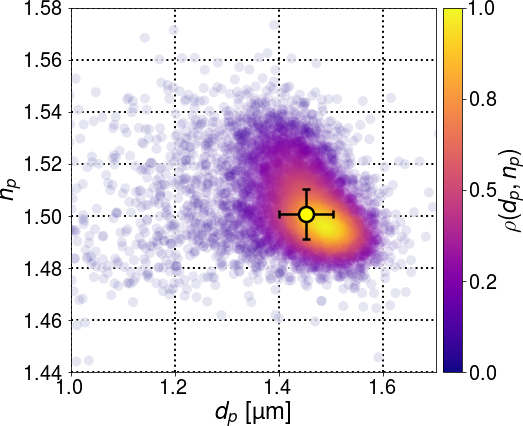
\includegraphics[width=0.5\textwidth]{distribution03}
    \caption{Holographic characterization data for a sample
    of \SI{1.5}{\um}-diameter TPM spheres synthesized with
    \SI{10}{\micro\liter} \ce{NH4OH} and 
    \SI{100}{\micro\liter} TPM at a mixing rate
    of $\Omega = \SI{700}{\per\minute}$.  Each 
    \DIFdelbeginFL \DIFdelFL{point
    }\DIFdelendFL \DIFaddbeginFL \DIFaddFL{of the \num{6935} points
    }\DIFaddendFL represents the diameter, $d_p$, and refractive index,
    $n_p$, of a single sphere and is colored by the relative
    density of measurements, $\rho(d_p, n_p)$.
    The cross is centered at the median values of the sample's
    characteristics and subtends their 
    median-absolute deviations.}
    \label{fig:typicalcharacterization}
\end{figure}

We perform holographic characterization measurements with a Spheryx xSight,
a commercial holographic particle characterization system.
The xSight draws a small sample of colloidal suspension through the
observation volume of an in-line holographic microscope where it is illuminated
\DIFdelbegin \DIFdel{with }\DIFdelend \DIFaddbegin \DIFadd{by }\DIFaddend a laser operating at a vacuum wavelength of \SI{532}{\nm}.
Light scattered by a colloidal particle interferes with the rest of the
beam in the focal plane of the microscope's objective lens.
The objective lens relays this interference pattern to a tube
lens that focuses it onto the sensor of a digital video camera.
The intensity of the recorded interference pattern is
a hologram of the particle that can be analyzed \DIFaddbegin \DIFadd{\mbox{%DIFAUXCMD
\cite{lee07a}
}\hspace{0pt}%DIFAUXCMD
}\DIFaddend to obtain information
about the particle's position and composition.
The instrument's analytical software fits each hologram 
to predictions of the Lorenz-Mie theory of light scattering
\DIFaddbegin \DIFadd{\mbox{%DIFAUXCMD
\cite{bohren83,mishchenko02,gouesbet11}
}\hspace{0pt}%DIFAUXCMD
}\DIFaddend to measure the associated particle's diameter and refractive index, as well as its
three-dimensional position relative to the center of the 
focal plane \cite{lee07a}.
Each particle is recorded and analyzed multiple times during its
transit through the observation volume\DIFdelbegin \DIFdel{to ensure reliable characterization results.
}\DIFdelend \DIFaddbegin \DIFadd{.
These time-resolved observations are linked into trajectories
using a maximum likelihood algorithm
\mbox{%DIFAUXCMD
\cite{crocker1996methods}}\hspace{0pt}%DIFAUXCMD
, both to map the particle's
transit through the sample volume and also to
combine multiple independent measurements 
of that particle's diameter and refractive index
for improved accuracy and precision \mbox{%DIFAUXCMD
\cite{cheong2009flow}}\hspace{0pt}%DIFAUXCMD
.
Typical measurements on micrometer-scale spheres yield
a particle's diameter with a precision of
\mbox{%DIFAUXCMD
\SI{5}{\nm} }\hspace{0pt}%DIFAUXCMD
and its refractive index to
within five parts per thousand
\mbox{%DIFAUXCMD
\cite{krishnatreya14,wang2016holographic}}\hspace{0pt}%DIFAUXCMD
.
Holographic analysis also yields the particle's
in-plane position to within a nanometer and its
axial position to within \mbox{%DIFAUXCMD
\SI{5}{\nm}
}\hspace{0pt}%DIFAUXCMD
\mbox{%DIFAUXCMD
\cite{cheong2009flow,krishnatreya14}}\hspace{0pt}%DIFAUXCMD
.
These measurements' accuracy and precision have
been validated with measurements on standard
particles \mbox{%DIFAUXCMD
\cite{lee07a,wang2016holographic}}\hspace{0pt}%DIFAUXCMD
,
by comparison with orthogonal techniques \mbox{%DIFAUXCMD
\cite{wang2016holographic}}\hspace{0pt}%DIFAUXCMD
,
and through analysis of well-understood physical processes
\mbox{%DIFAUXCMD
\cite{krishnatreya14}}\hspace{0pt}%DIFAUXCMD
.
}\DIFaddend 

\DIFaddbegin \DIFadd{Originally demonstrated with dispersions of model
colloidal spheres \mbox{%DIFAUXCMD
\cite{lee07a}}\hspace{0pt}%DIFAUXCMD
,
holographic particle characterization has been
applied successfully to porous particles \mbox{%DIFAUXCMD
\cite{cheong11}}\hspace{0pt}%DIFAUXCMD
,
dimpled spheres \mbox{%DIFAUXCMD
\cite{hannel2015holographic}}\hspace{0pt}%DIFAUXCMD
,
and fractal aggregates \mbox{%DIFAUXCMD
\cite{wang2016fractal}}\hspace{0pt}%DIFAUXCMD
.
Time-resolved holographic characterization has been used to
monitor the growth of colloidal polydimethylsiloxane (PDMS)
spheres \mbox{%DIFAUXCMD
\cite{wang15}}\hspace{0pt}%DIFAUXCMD
, the response of colloidal
sensors to changing environmental conditions
\mbox{%DIFAUXCMD
\cite{wang2015stimulus} }\hspace{0pt}%DIFAUXCMD
and molecular binding
to the surface of functionalized beads \mbox{%DIFAUXCMD
\cite{cheong2009flow}}\hspace{0pt}%DIFAUXCMD
.
Practical applications include monitoring protein aggregation 
in biopharmaceuticals
\mbox{%DIFAUXCMD
\cite{wang2016holographic,kasimbeg2019holographic}}\hspace{0pt}%DIFAUXCMD
, 
nanoparticle agglomeration in semiconductor polishing
slurries \mbox{%DIFAUXCMD
\cite{cheong17} }\hspace{0pt}%DIFAUXCMD
and oil droplet concentration in
wastewater \mbox{%DIFAUXCMD
\cite{philips2017holographic}}\hspace{0pt}%DIFAUXCMD
.
}

\DIFaddend xSight measurements are limited to particle concentrations
below \SI{E6}{\per\milli\liter} to minimize interference
of overlapping single-particle holograms.
TPM synthesis, however,
produces samples with number densities of \SI{E10}{\per\milli\liter}.
We therefore
dilute each sample by a factor of \num{E4}
with deionized water before analysis.
This should not affect the particles'
properties because oligomerized TPM droplets and 
polymerized spheres are hydrophobic \cite{vanderwel17}.

We analyze each sample by pipetting \SI{100}{\micro\liter} of the diluted
dispersion into an xCell microfluidic sample cell and loading the xCell into the xSight.
The xSight draws \SI{3}{\micro\liter} of the fluid through
the xCell's \SI{50}{\um} deep observation volume.
A ten-minute measurement provides
\DIFdelbegin \DIFdel{us with
}\DIFdelend characterization data for a few thousand colloidal spheres per sample.
A typical example is presented in Fig.~\ref{fig:typicalcharacterization}.
\DIFaddbegin \DIFadd{Each point in this plot represents the measured diameter, $d_p$,
and refractive index, $n_p$, of a single particle, averaged over
multiple measurements. Points are
colored by the relative density of observations.
This coloring reveal a peak in the distribution at $d_p = \SI{1.5}{\um}$
and $n_p = \num{1.495}$. The cross superimposed on the plot indicates
the median particle diameter and median refractive index, together
with the median absolute deviation in those properties.
The spread in measured properties is much larger than the
measurement uncertainty, and so represents
the polydispersity in the sample's actual properties.
}\DIFaddend 

\begin{figure}
  \centering
  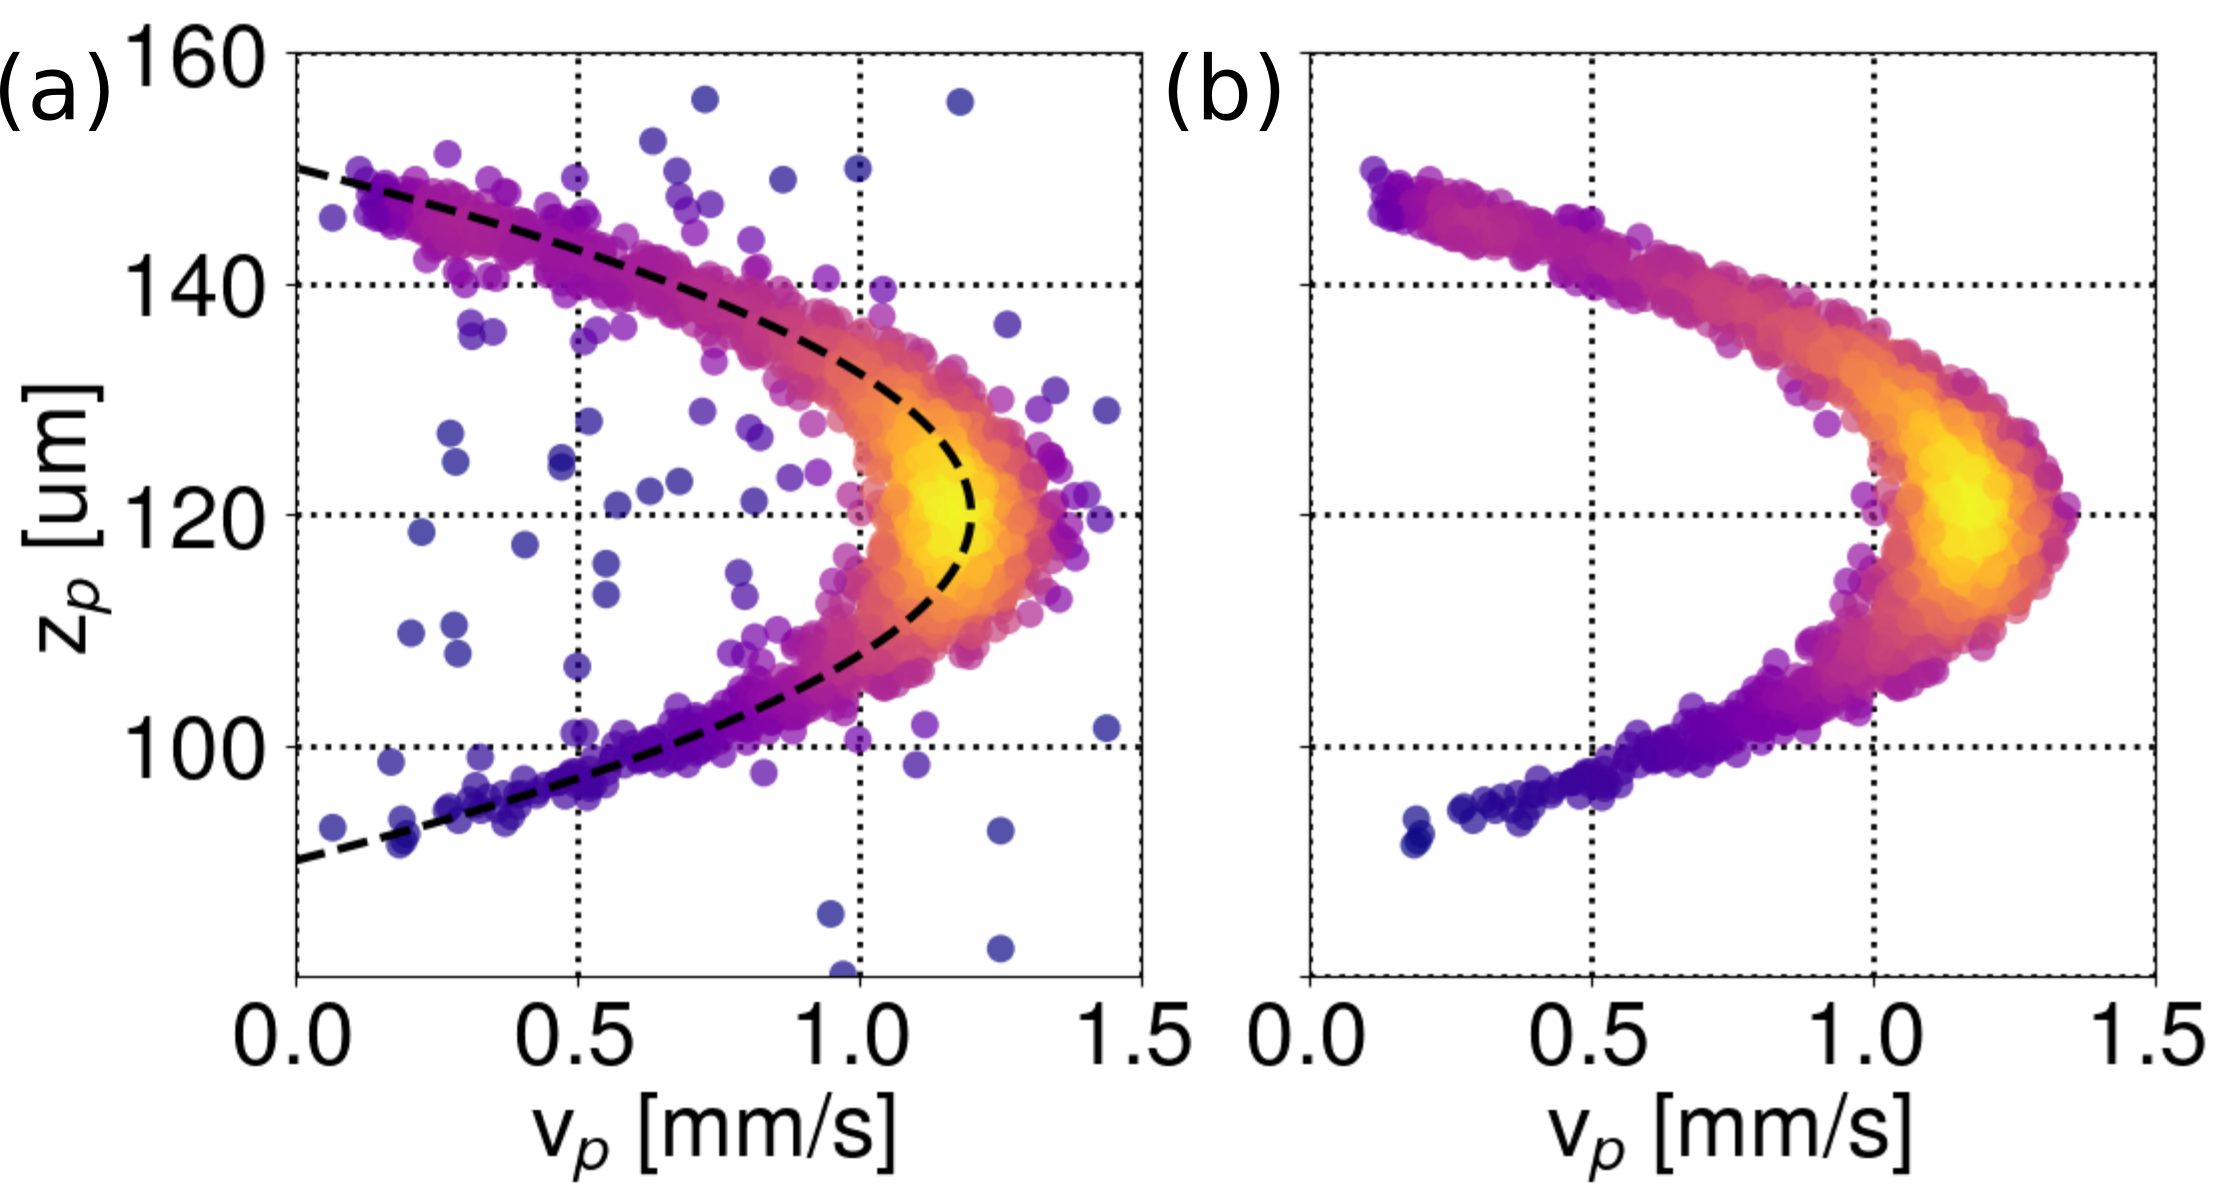
\includegraphics[width=0.8\textwidth]{velocity_plots}
  \caption{(a) Scatter plot of particle speed, 
    $v_p$, as a function of
    height $z_p$, above the focal plane.  Each dot represents
    tracking data for a single particle and is colored
    by the density of observations. The dashed blue curve
    is a fit to a parabola.
    (b) Filtered results.}
  \label{fig:flow_prof}
\end{figure}

\DIFdelbegin \DIFdel{Holographic tracking data }\DIFdelend \DIFaddbegin \DIFadd{The measured trajectories of colloidal particles 
}\DIFaddend can be used to monitor
the success of a measurement by mapping the
Poiseuille flow profile within the xCell microfluidic
channel \DIFdelbegin \DIFdel{\mbox{%DIFAUXCMD
\cite{cheong10a}}\hspace{0pt}%DIFAUXCMD
}\DIFdelend \DIFaddbegin \DIFadd{\mbox{%DIFAUXCMD
\cite{cheong2009flow,cheong10a}}\hspace{0pt}%DIFAUXCMD
}\DIFaddend .
Each point in Fig.~\ref{fig:flow_prof}(a)
represents the \DIFdelbegin \DIFdel{measured }\DIFdelend speed, $v_p(z_p)$, for a single
particle's transit at its mean axial position, $z_p$\DIFdelbegin \DIFdel{,
averaged over
its trajectory through the observation volume.
The solid }\DIFdelend \DIFaddbegin \DIFadd{.
The width of the observed distribution of transit speeds
is dominated by variations in the pump speed over
the \mbox{%DIFAUXCMD
\SI{10}{\minute} }\hspace{0pt}%DIFAUXCMD
course of the measurement.
These variations do not affect the precision or accuracy
of characterization measurements because 
the flow speed is always low enough to avoid artifacts
due to motion blurring \mbox{%DIFAUXCMD
\cite{cheong2009flow,dixon2011holographic}}\hspace{0pt}%DIFAUXCMD
.
The dashed }\DIFaddend curve in Fig.~\ref{fig:flow_prof}(\DIFdelbegin \DIFdel{b}\DIFdelend \DIFaddbegin \DIFadd{a}\DIFaddend ) is a fit to a
\DIFdelbegin \DIFdel{parabola}\DIFdelend \DIFaddbegin \DIFadd{the expected parabolic flow profile}\DIFaddend . 
Extrapolating this fit to \DIFdelbegin \DIFdel{$v(z)=0$ }\DIFdelend \DIFaddbegin \DIFadd{$v(z) = 0$ }\DIFaddend yields estimates
for the axial positions of the channel's walls, assuming
no-slip boundary conditions.
\DIFaddbegin \DIFadd{The measured \mbox{%DIFAUXCMD
\SI{51}{\um} }\hspace{0pt}%DIFAUXCMD
range is consistent with
the xCell's nominal channel depth.
}\DIFaddend Because the particle's axial position is measured
relative to the microscope's focal plane,
\DIFdelbegin \DIFdel{this result
}\DIFdelend \DIFaddbegin \DIFadd{the measured range of $z_p$
}\DIFaddend can be used to confirm that the xCell is seated
properly within the xSight during measurement.

Most observations fall neatly onto the parabolic profile.
Some, however, deviate markedly, presumably because
of tracking errors \DIFdelbegin \DIFdel{due to overlapping holograms.
The associated characterization data also }\DIFdelend \DIFaddbegin \DIFadd{that result in particles being
misidentified in a sequence of holograms.
Tracking errors are more common in holograms
containing multiple particles, particularly when
faster-moving particles near the midplane of the
channel overtake slower-moving particles near
the walls.
Characterization data obtained from such faulty tracks
}\DIFaddend are likely to \DIFdelbegin \DIFdel{be unreliable}\DIFdelend \DIFaddbegin \DIFadd{combine results from different particles
rather than reflecting the properties of just one particle}\DIFaddend .
We therefore reject any features that deviate from
the parabolic profile by more than one median absolute deviation,
as depicted in Fig.~\ref{fig:flow_prof}(b).
\DIFaddbegin \DIFadd{In this case, \num{72} out of \num{6807} trajectories
were cut.
}\DIFaddend The remaining results are used
to characterize the sample\DIFdelbegin \DIFdel{.
}\DIFdelend \DIFaddbegin \DIFadd{, as is the case
in Fig.~\ref{fig:typicalcharacterization}.
}\DIFaddend 

\subsection{Orthogonal validation methods}
\label{sec:orthogonalmethods}

Holographic particle characterization is a comparatively new technique
and is not yet widely adopted. We therefore validate results from
holographic particle characterization with 
orthogonal measurement techniques.
Specifically, we use scanning electron microscopy to provide baseline estimates for the
particles' diameters and Abbe refractometry to measure their refractive indexes.

\DIFaddbegin \subsubsection{\DIFadd{Scanning electron microscopy}}

\DIFaddend \begin{figure}
  \centering
  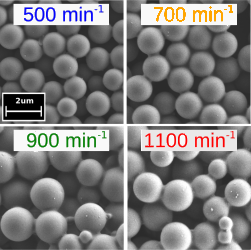
\includegraphics[width=0.5\textwidth]{semimages03}
  \caption{SEM images of polymerized TPM spheres
    prepared at four different stirring rates.}
  \label{fig:semimages}
\end{figure}

Each sample of polymerized spheres was imaged with a 
field emission scanning electron microscope
(MERLIN SEM, Carl Zeiss).
Typical images are presented in Fig.~\ref{fig:semimages}.
SEM images provide a visual check of the spheres' surface
texture and can be used to estimate their mean
diameter and polydispersity.
While a well calibrated scanning
electron microscope provides \num{1} to \SI{10}{\nm} spatial resolution, sample
preparation, particularly exposure to vacuum and sputter coating, can shrink or 
even swell the sample \cite{yamada85,jung02}.
TPM emulsion droplets are \DIFaddbegin \DIFadd{fluid and so
are }\DIFaddend not amenable to SEM analysis.

\DIFaddbegin \DIFadd{The diameter of an individual sphere is obtained 
by analyzing its image with ImageJ \mbox{%DIFAUXCMD
\cite{schindelin2015imagej}}\hspace{0pt}%DIFAUXCMD
, specifically by
drawing a tight-fitting oval around its image and
computing the average of the oval's major and minor axes.
The distribution of sphere diameters is
estimated by analyzing \num{50} spheres' images
for each sample.
}

\subsubsection{\DIFadd{Abbe refractometry}}

\DIFaddend \begin{figure}
  \centering
  \DIFdelbeginFL %DIFDELCMD < 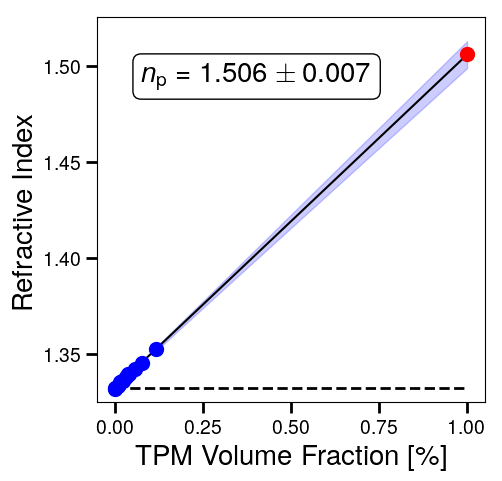
\includegraphics[width=0.5\textwidth]{abbe}
%DIFDELCMD <   %%%
\DIFdelendFL \DIFaddbeginFL 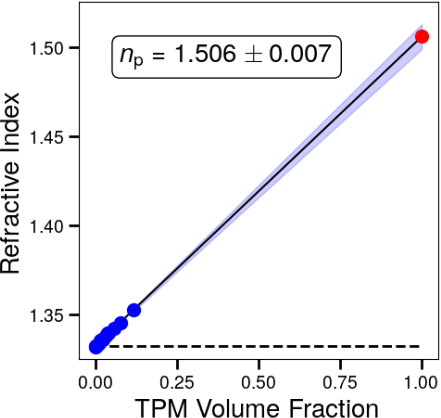
\includegraphics[width=0.5\textwidth]{abbe02}
  \DIFaddendFL \caption{Estimating $n_p$ through refractometry.
    Discrete (blue) points reflect the refractive index,
    $n(\phi)$, of \num{12} suspensions as a function of volume fraction,
    $\phi$. Linear extrapolation to $\phi = 1$
    yields an estimate for the refractive index of the dispersed phase,
    $n_p$, represented as a red dot.
    The (blue) shaded region represents the \SI{95}{\percent}
    prediction interval for the extrapolation.
    The lower dashed line represents the refractive index of water at
    \SI{532}{\nm}.}
  \label{fig:abbe}
\end{figure}

We estimate the refractive index of the TPM particles
by suspending them in water and measuring the mean refractive index of
the suspensions,
$n(\phi)$,
as a function of the particles' volume fraction, $\phi$.
Linearly extrapolating  to $\phi = 1$
yields an estimate for the spheres' refractive index,
$n_p$,
in their native medium at room temperature \SI{21.5}{\celsius}
\cite{alexander81}.
Figure~\ref{fig:abbe} shows an application
of this technique to two similarly prepared
samples of TPM spheres.
\DIFdelbegin \DIFdel{Each sample was }\DIFdelend \DIFaddbegin 

\DIFadd{The initial number density of particles in each
sample is obtained with the xSight by counting
the particles in \mbox{%DIFAUXCMD
\SI{3}{\micro\liter} }\hspace{0pt}%DIFAUXCMD
of fluid.
This approach yields particle concentrations with
an accuracy of \mbox{%DIFAUXCMD
\SI{10}{\percent} }\hspace{0pt}%DIFAUXCMD
in the range
from \mbox{%DIFAUXCMD
\SI{e3}{particles\per\milli\liter}
}\hspace{0pt}%DIFAUXCMD
to \mbox{%DIFAUXCMD
\SI{e7}{particles\per\milli\liter} }\hspace{0pt}%DIFAUXCMD
\mbox{%DIFAUXCMD
\cite{wang2016holographic}}\hspace{0pt}%DIFAUXCMD
.
Each sample is }\DIFaddend diluted to \num{5} different volume 
fractions to provide a total of \num{12}
different suspensions, including the two stock samples.
The refractive index of each
suspension was measured with an Abbe refractometer
at room temperature \SI{21.5}{\degreeCelsius}.
Linear extrapolation yields
$n_p = \num{1.506(7)}$ with \SI{95}{\percent} confidence.
This range includes uncertainty in the samples
volume fractions as well as any differences between the
two samples.
\DIFaddbegin \DIFadd{This result demonstrates both the reproducibility of the
synthesis and the reproducibility of this measurement
technique.
}\DIFaddend 

This method is complementary to the approach used
by van der Wel, \emph{et al.},
who index matched their particles to a solution of
pyridine ($n=1.509$) and \num{2}-ethylhexyl
\num{4}-methoxycinnamate ($n = \num{1.545}$)
and identified the refractive index of the particles
with that of the best index matching solution \cite{vanderwel17}.
They report the refractive index to be between 
\num{1.512} and \num{1.513},
presumably at a wavelength of \SI{589}{\nm}.

\subsection{Optimization strategies}
\label{sec:optimizationstrategies}

The immediate goal of this study is to design
a synthesis protocol that reproducibly 
yields TPM spheres with a selected size and
the smallest degree of polydispersity in size.
Factors governing size selection include
ammonia concentration, emulsion stoichiometry,
and mixing conditions.
These factors determine the nucleation rate of oligomer
droplets, the rate and duration of growth, 
and the homogeneity of these processes, respectively.

The choice of free-radical initiator \DIFdelbegin \DIFdel{should }\DIFdelend \DIFaddbegin \DIFadd{does }\DIFaddend not affect
the size distribution of the oligomer droplets, but
may influence the course of polymerization, and thus
the density and size of the final spheres.
Oil-soluble initiators might be expected to
polymerize the spheres uniformly thereby
shrinking the spheres as the material becomes more
dense.
Water-soluble initiators, by contrast, might
polymerize the spheres from the surface inward,
perhaps inhibiting shrinkage and producing a 
larger and less dense product.

To guide protocol design, we first monitor
the effect of mixing conditions on size selection
during droplet formation.
Using holographic characterization data to 
monitor polymerization speeds the optimization process
by identifying when processing has run to completion.
We then use the optimal mixing conditions for
a binary search through parameter space of
ammonia concentration and TPM stoichiometry.
Finally, we assess the influence of initiator
choice on particle properties.

\section{Results and Discussion}
\label{sec:results}

Each holographic particle characterization
measurement
requires roughly \SI{15}{\minute} including
sample preparation and yields 
a comprehensive view of the joint
distribution of the sizes and refractive
indexes of the particle in the sample.
Orthogonal techniques yield information
about the \DIFdelbegin \DIFdel{size distribution or about
the refractive index distribution separately.
We therefore use these techniques to validate
size data and compositiondata independently}\DIFdelend \DIFaddbegin \DIFadd{particles' size distribution and
refractive index separately}\DIFaddend .
\DIFaddbegin \DIFadd{They cannot identify correlations between
size and composition.
We therefore average holographic characterization
data over the complementary characteristic when
comparing with orthogonal techniques.
}\DIFaddend 

\subsection{Effect of stirring rate on particle size}
\label{sec:stir}

Stirring the sample while the oligomers condense into droplets promotes
homogeneous nucleation by uniformly dispersing the hydrolyzed monomer
and droplet nuclei, thereby ensuring that all droplets grow under
comparable conditions.
Beyond simply mixing the sample, however, stirring creates shear
forces \cite{halasz2007vortex} that can alter droplets' size
distribution \DIFdelbegin \DIFdel{\mbox{%DIFAUXCMD
\cite{oles1992shear,eggersdorfer2010fragmentation}}\hspace{0pt}%DIFAUXCMD
}\DIFdelend \DIFaddbegin \DIFadd{\mbox{%DIFAUXCMD
\cite{oles1992shear,eggersdorfer2010fragmentation,yeung2003shear}}\hspace{0pt}%DIFAUXCMD
}\DIFaddend .
The overall effect of stir rate on the resulting particle size
is best assessed experimentally.

Figure~\ref{fig:sizedistribution} summarizes how
stirring rate influences the size
of TPM spheres for a given set of synthesis conditions.
The four emulsions represented in this plot
were produced in identical cylindrical 
vials with identical stir bars. 
Each vial was charged with
\DIFdelbegin \DIFdel{\mbox{%DIFAUXCMD
\SI{15}{\micro\liter} }\hspace{0pt}%DIFAUXCMD
}\DIFdelend \DIFaddbegin \DIFadd{\mbox{%DIFAUXCMD
\SI{15.0(3)}{\micro\liter} }\hspace{0pt}%DIFAUXCMD
}\DIFaddend of \SI{29}{\percent} ammonia 
(\SI{29.3}{\percent} \ce{NH3}(aq) by \ce{HCl} titration) 
\DIFaddbegin \DIFadd{using an Eppendorf Research plus pipette, }\DIFaddend followed by
\SI{200}{\micro\liter} of TPM monomer and was immediately
brought up to \SI{5}{\milli\liter} with DI water.
These conditions yield $\text{pH} = \num{11.0}$ and
$[\ce{TPM}] = \SI{0.16}{M}$.
The four samples were stirred for \SI{2}{\hour}
using magnetic stir plates set at \num{500}, \num{700}, \num{900}, and
\SI{1100}{\per\minute}. 
The resulting droplets were polymerized by adding an excess (\SI{1}{mg}) of AIBN
as a radical initiator and
heating the sample to \SI{80}{\celsius} for \SI{2}{\hour}.
% Explanation: 1 mg AIBN corresponds to 3.7e18 molecules at 164 g/mol.
% This can be compared with roughly 5e12 droplets in the 5 mL sample,
% which means that we have roughly a million initiator molecules per droplet.
These samples then were analyzed by both HPC and SEM.

The mixing conditions are set by the geometry of the vial, the shape
of the stir rod, and the stir rate. The \SI{12}{\milli\liter}
cylindrical vials 
have an inner diameter of \SI{16}{\milli\meter} and a height of \SI{60}{\milli\meter}.
Each \SI{5}{\milli\liter} sample filled approximately one third of the cylinder's volume.
Each pill-shaped magnetic stir rod has a long axis length of \SI{12}{\milli\meter} 
and short axis length of \SI{7}{\milli\meter}.
The \DIFaddbegin \DIFadd{nature of the flow in the vial can be gauged with
the }\DIFaddend dimensionless impeller Reynolds number\DIFdelbegin \DIFdel{distinguishes turbulent and laminar flows and is given as
}\DIFdelend \DIFaddbegin \DIFadd{,
}\DIFaddend \begin{equation}
    N_{Re} = \frac{\Omega d^2 \rho}{\mu},
\end{equation}
where $\Omega$ is the rotation speed in rotations per second, 
$d$ is the impeller diameter, and $\rho$ and $\mu$ refer to the
density and dynamic viscosity of water, respectively.
\DIFdelbegin \DIFdel{Therefore }\DIFdelend \DIFaddbegin \DIFadd{The transition from laminar flow to turbulent flow occurs for
$N_{Re} > \num{1000}$.
In our system, }\DIFaddend the impeller Reynolds number \DIFdelbegin \DIFdel{varies }\DIFdelend \DIFaddbegin \DIFadd{ranges }\DIFaddend from
\num{3200} at a stir rate of \SI{500}{\per\minute}
to \num{7000} at \SI{1100}{\per\minute}\DIFdelbegin \DIFdel{.
This means that the tangential flow is turbulent }\DIFdelend \DIFaddbegin \DIFadd{,
and so is turbulent \mbox{%DIFAUXCMD
\cite{halasz2007vortex}}\hspace{0pt}%DIFAUXCMD
.
The meniscus of the driven vortex ranges in depth
from \mbox{%DIFAUXCMD
\SI{5}{\mm} }\hspace{0pt}%DIFAUXCMD
at \mbox{%DIFAUXCMD
\SI{500}{\per\minute}
}\hspace{0pt}%DIFAUXCMD
to \mbox{%DIFAUXCMD
\SI{20}{\mm} }\hspace{0pt}%DIFAUXCMD
at \mbox{%DIFAUXCMD
\SI{1100}{\per\minute}}\hspace{0pt}%DIFAUXCMD
, and does not reach
the stir bar until \mbox{%DIFAUXCMD
\SI{2000}{\per\minute}}\hspace{0pt}%DIFAUXCMD
.
These considerations suggest that samples should be
well mixed }\DIFaddend over the entire range \DIFdelbegin \DIFdel{\mbox{%DIFAUXCMD
\cite{halasz2007vortex}}\hspace{0pt}%DIFAUXCMD
}\DIFdelend \DIFaddbegin \DIFadd{of stirring rates,
the principal difference among them being the intensity of the shear forces
encountered by the dispersed droplets}\DIFaddend .

The results in Fig.~\ref{fig:sizedistribution}
reveal that the smallest mean particle size is
obtained at the lowest stirring speeds.
This surprising observation
runs counter to the usual trend \cite{oles1992shear,eggersdorfer2010fragmentation}
in emulsion polymerization
\cite{chern06}
and suspension polymerization
\cite{arshady92}.
Increasing stirring speed also increases the particles'
polydispersity, particularly increasing the proportion of undersized particles.
\DIFaddbegin \DIFadd{It is possible that increasing shear rate favors 
collision-induced droplet coalescence in this system
\mbox{%DIFAUXCMD
\cite{yeung2003shear}}\hspace{0pt}%DIFAUXCMD
.
}\DIFaddend The samples' \DIFdelbegin \DIFdel{mean }\DIFdelend \DIFaddbegin \DIFadd{median }\DIFaddend diameters, $\avg{d_{\text{p}}}$,
are reported in Table~\ref{table:sem_data} together
with their standard deviations, $\sigma_{d_{\text{p}}}$.

\DIFdelbegin \DIFdel{Size distributions obtained holographically are consistent with results 
of SEM analysis on the same samples, including
the images in Fig.~\ref{fig:semimages}.
The mean sphere diameter is estimated by analyzing \num{50} spheres' images using ImageJ \mbox{%DIFAUXCMD
\cite{mazzoli12}}\hspace{0pt}%DIFAUXCMD
. %DIF <  Find better citation?
The diameter of an individual sphere is obtained 
drawing a tight-fitting oval around its image;
the average of each oval's minor and major axes provides an estimate for the
associated sphere's diameter.
The resulting histograms of particle diameters
also are plotted in Fig.~\ref{fig:sizedistribution}.
}\DIFdelend
\begin{figure}[!t]
  \centering
  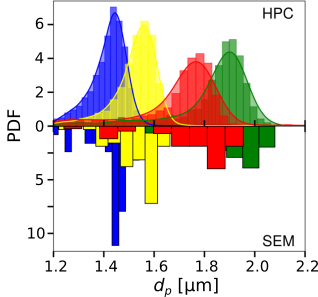
\includegraphics[width=0.5\textwidth]{sizedistributions03}
  \caption{\DIFaddFL{Probability distribution function (PDF) for 
    sphere diameters as measured by
    holographic particle characterization (HPC) and by SEM for
    samples that were stirred at 
    \num{500} (blue), 
    \num{700} (yellow), 
    \num{900} (green), 
    and \mbox{%DIFAUXCMD
\SI{1100}{\per\minute} }\hspace{0pt}%DIFAUXCMD
(red).
    HPC results are projections of joint
    distributions such as the example in
    Fig.~\ref{fig:typicalcharacterization}
    and each summarize several thousand single-particle measurements.
    Histograms of SEM results were compiled from
    images of dried samples such as the
    examples in Fig.~\ref{fig:semimages}.}}
  \label{fig:sizedistribution}
\end{figure}


\DIFdelbegin \DIFdel{Based on the outcome of this survey, we synthesize
the remainder of the particles in this study
at a stirring rate of \mbox{%DIFAUXCMD
\SI{700}{\per\minute}}\hspace{0pt}%DIFAUXCMD
,
which yields particles with the smallest
relative polydispersity.
}%DIFDELCMD < 

%DIFDELCMD < \begin{table}[!t]
%DIFDELCMD < %%%
\DIFdelendFL \DIFaddbeginFL \begin{table}[hb]
\DIFaddendFL \centering
\caption{Median size and standard deviation of TPM spheres
  measured by SEM analysis 
  and holographically for each of the four stir rates.}
\begin{tabular}{rrrrr}
\hline
\hline
$\Omega~[\si{\per\minute}]$ & \num{500} & \num{700}& \num{900} & \num{1100} \\
\hline
$\avg{d_p}_{\text{SEM}}~[\si{\um}]$ & 1.45 & 1.56 & 1.92 & 1.75 \\ 
$\sigma_{d_p, \text{SEM}}~[\si{\um}]$ & 0.12 & 0.13 & 0.28 & 0.32 \\ 
$\avg{d_p}_{\text{HPC}}~[\si{\um}]$ & 1.43 & 1.54 & 1.88 & 1.73 \\ 
$\sigma_{d_p, \text{HPC}}~[\si{\um}]$ & 0.04 & 0.05 & 0.06 & 0.08 \\ 
\hline \hline
\end{tabular}
\label{table:sem_data}
\end{table}

\DIFaddbegin \DIFadd{Size distributions obtained holographically are consistent with results of SEM analysis on the same samples, including
the images in Fig.~\ref{fig:semimages}.
These results
also are plotted in Fig.~\ref{fig:sizedistribution}
and reported in Table~\ref{table:sem_data}.
For all samples, the median particle diameter
obtained holographically agrees with the median
SEM result to within \mbox{%DIFAUXCMD
\SI{40}{\nm}}\hspace{0pt}%DIFAUXCMD
, which is smaller
than the sample standard deviation.
This agreement supports our use of HPC for rapid
sample characterization.
}

\DIFaddend Although unpolymerized droplets are not amenable to SEM analysis,
they can be by analyzed holographically.
Figure~\ref{fig:jointspeed} presents the median size and refractive index
of TPM emulsion droplets prepared at the four stirring rates,
both before and after polymerization.
Overall the influence of polymerization on median droplet diameter is
consistent with the \SI{2}{\percent} reduction in size reported by
van der Wel, \emph{et al.}
based on dynamic light scattering \cite{vanderwel17}.

\DIFaddbegin \DIFadd{Based on the outcome of this survey, we synthesize
the remainder of the particles in this study
at a stirring rate of \mbox{%DIFAUXCMD
\SI{700}{\per\minute}}\hspace{0pt}%DIFAUXCMD
,
which reproducibly yields particles with
\mbox{%DIFAUXCMD
\SI{3}{\percent} }\hspace{0pt}%DIFAUXCMD
relative polydispersity in diameter.
}

\DIFaddend \subsection{Effect of stirring rate on refractive index}
\label{sec:stirindex}

\begin{figure}
  \centering
  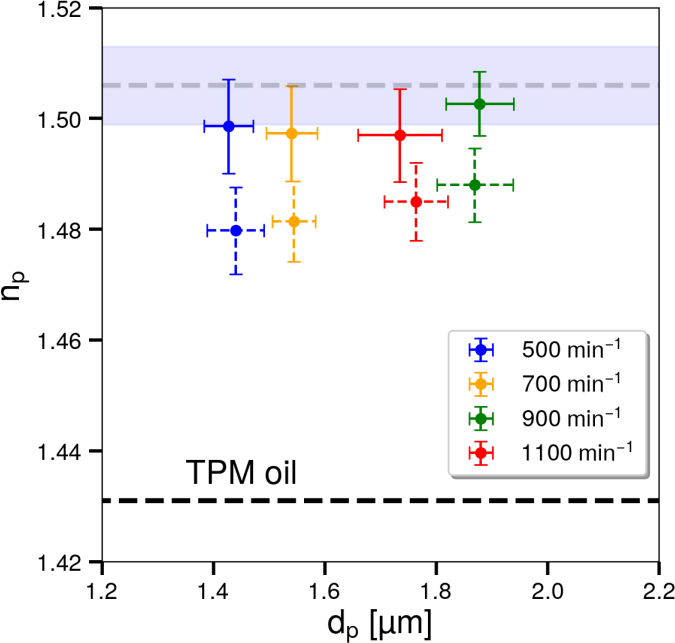
\includegraphics[width=0.5\textwidth]{jointspeed}
  \caption{Holographic characterization of emulsion droplets
    (dashed lines) and polymerized spheres (solid lines)
    stirred at \num{4} different rates.
    Filled circles represents the median diameter and refractive index
    for one sample.  Error bars represent one median absolute 
    deviation from the median.
    The dashed black line represents the refractive index of monomeric
    TPM oil.
    The dashed gray line represents the refractive index for polymerized
    TPM spheres obtained with conventional refractometry, including
    the \SI{95}{\percent} prediction interval.}
  \label{fig:jointspeed}
\end{figure}

Figure~\ref{fig:jointspeed} summarizes holographic characterization
results for the influence of stirring rate on the properties of TPM
emulsions and their associated polymerized \DIFdelbegin \DIFdel{dispersion}\DIFdelend \DIFaddbegin \DIFadd{spheres}\DIFaddend .
Each dot represents the median size and refractive index for \DIFdelbegin \DIFdel{the associated }\DIFdelend \DIFaddbegin \DIFadd{one }\DIFaddend sample.
Error bars represent the median absolute deviations of those properties.

Whereas stirring has a substantial influence on droplet size,
its effect on refractive index is slight\DIFdelbegin \DIFdel{at most}\DIFdelend .
This is reasonable because the refractive index reflects
the composition of the condensed phase, which should not
\DIFdelbegin \DIFdel{be substantially influenced by }\DIFdelend \DIFaddbegin \DIFadd{vary substantially with }\DIFaddend local flow conditions.
\DIFdelbegin \DIFdel{The polymerized }\DIFdelend \DIFaddbegin \DIFadd{Polymerized }\DIFaddend spheres have an average refractive index of
$n_p = \num{1.501(9)}$, which is consistent with \DIFdelbegin \DIFdel{conventional
refractometry.
The unpolymerized }\DIFdelend \DIFaddbegin \DIFadd{the value
obtained by Abbe refractometry.
}

\DIFadd{Unpolymerized }\DIFaddend emulsion droplets have a systematically 
lower refractive index \DIFdelbegin \DIFdel{.
}\DIFdelend \DIFaddbegin \DIFadd{than polymerized spheres
}\DIFaddend Polymerization changes the chemical makeup of the droplet and
generally increases the density\DIFaddbegin \DIFadd{. }\DIFaddend % FIXME: Add citation.
\DIFdelbegin \DIFdel{and so }\DIFdelend \DIFaddbegin \DIFadd{Both effects }\DIFaddend might reasonably account for the observed change in refractive index.

\DIFdelbegin \DIFdel{The refractive indexes of }\DIFdelend \DIFaddbegin \DIFadd{Oligomerized }\DIFaddend TPM droplets and polymerized spheres both
\DIFdelbegin \DIFdel{substantially exceed that of }\DIFdelend \DIFaddbegin \DIFadd{have higher refractive indexes than }\DIFaddend bulk TPM oil, which is indicated by
a dashed line in Fig.~\ref{fig:jointspeed}.
Hydrolysis and oligomerization account for a refractive
index shift of roughly \num{0.05} and polymerization accounts for the remaining
increase of \num{0.02}.

\subsection{Monitoring polymerization}
\label{sec:monitoring}

The \DIFdelbegin \DIFdel{small but clearly resolved 
change in }\DIFdelend \DIFaddbegin \DIFadd{data in Fig.~\ref{fig:heat_size_time}
illustrate how changes in }\DIFaddend droplet size and refractive index can be
used to monitor the progress of polymerization.
This is useful both for ensuring that polymerization has run
to completion before analysis, and also for minimizing the
time required for combinatorial studies of processing choices.
\DIFdelbegin %DIFDELCMD < 

%DIFDELCMD < %%%
\DIFdel{Figure~\ref{fig:heat_size_time} illustrates how
holographic characterization can be used to monitor
droplet polymerization.  }\DIFdelend This sample consists of an emulsion of TPM droplets \DIFdelbegin \DIFdel{and 
the initiatorAIBN}\DIFdelend \DIFaddbegin \DIFadd{undergoing
polymerization with AIBN as the initiator}\DIFaddend .
The suspension is continuously stirred at 
\SI{1100}{\per\minute}
and is thermally coupled to a heat bath set at \SI{80}{\degreeCelsius}.
Starting when the initiator is added,
we draw \DIFdelbegin \DIFdel{\mbox{%DIFAUXCMD
\SI{1}{\ul} }\hspace{0pt}%DIFAUXCMD
}\DIFdelend \DIFaddbegin \DIFadd{\mbox{%DIFAUXCMD
\SI{1}{\micro\liter} }\hspace{0pt}%DIFAUXCMD
}\DIFaddend of the suspension after 
\num{5}, \num{10}, \num{15},
\num{20}, \num{40}, \SI{60}{\minute}.
Each aliquot is added immediately 
to \SI{10}{\milli\liter} of room temperature deionized water
to arrest polymerization through thermal quenching.
The diluted sample then is transferred to the xSight
for analysis.

\begin{figure}
  \centering
  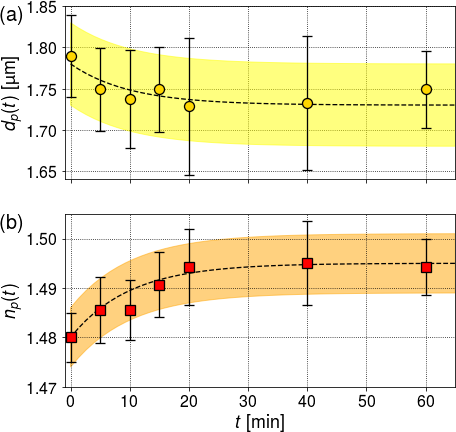
\includegraphics[width=0.5\textwidth]{polymerization04}
  \caption{Particle properties after heat bath exposure times
    of \num{5}, \num{10}, \num{15}, \num{20}, \num{40}, and 
    \SI{60}{\min}.
    (a) The average size and (b) refractive index of particles as a function
    of heat bath exposure time.
    Error bars indicate a single median absolute deviation
    of the associated property.}
  \label{fig:heat_size_time}
\end{figure}

The median diameter of the TPM droplets plotted
in Fig.~\ref{fig:heat_size_time}(a)
decreases by \SI{2}{\percent} on average
during polymerization.
Although this is \DIFdelbegin \DIFdel{well }\DIFdelend within the
measured polydispersity of each sample, 
it is consistent with the \SI{7}{\percent} reduction
in volume reported in Ref.~[{\hspace*{-1ex}\citenum{vanderwel17}}].
The change in size is correlated with 
a simultaneous increase in the refractive index
from \num{1.485} to \num{1.495} that is
plotted in Fig.~\ref{fig:heat_size_time}(b).
\DIFdelbegin %DIFDELCMD < 

%DIFDELCMD < %%%
\DIFdelend Dashed curves in Fig.~\ref{fig:heat_size_time}
are exponentials with a \SI{10}{\minute} characteristic
time that are superimposed on the data as a guide
to the eye.
Changes in dispersion properties have largely run
their course in \SI{20}{\minute}.
\DIFdelbegin \DIFdel{All four initiators are active for this period with
}\DIFdelend \DIFaddbegin 

\DIFadd{All four free-radical initiators have }\DIFaddend half-lives
at \SI{80}{\degreeCelsius} \DIFdelbegin \DIFdel{of \mbox{%DIFAUXCMD
\SI{1.8}{\hour}
}\hspace{0pt}%DIFAUXCMD
(APS\mbox{%DIFAUXCMD
\cite{borisov2015kinetic}}\hspace{0pt}%DIFAUXCMD
),
\mbox{%DIFAUXCMD
\SI{2}{\hour} }\hspace{0pt}%DIFAUXCMD
(KPS \mbox{%DIFAUXCMD
\cite{beylerian2002kinetics}}\hspace{0pt}%DIFAUXCMD
),
\mbox{%DIFAUXCMD
\SI{6}{\hour} }\hspace{0pt}%DIFAUXCMD
(AIBN ) and \mbox{%DIFAUXCMD
\SI{30}{\hour}
}\hspace{0pt}%DIFAUXCMD
(ACHN )}\DIFdelend \DIFaddbegin \DIFadd{that are substantially longer
than the time required to polymerize the droplets.
The shortest-lived initiator is APS, with a half-life
of \mbox{%DIFAUXCMD
\SI{1.8}{\hour} }\hspace{0pt}%DIFAUXCMD
\mbox{%DIFAUXCMD
\cite{borisov2015kinetic}}\hspace{0pt}%DIFAUXCMD
.
KPS has a half-life of \mbox{%DIFAUXCMD
\SI{2}{\hour} }\hspace{0pt}%DIFAUXCMD
\mbox{%DIFAUXCMD
\cite{beylerian2002kinetics}}\hspace{0pt}%DIFAUXCMD
,
AIBN has a half-life of
\mbox{%DIFAUXCMD
\SI{6}{\hour} }\hspace{0pt}%DIFAUXCMD
and ACHN has a half-life of \mbox{%DIFAUXCMD
\SI{30}{\hour}}\hspace{0pt}%DIFAUXCMD
}\DIFaddend .
The results in Fig.~\ref{fig:heat_size_time} therefore
suggest that heating for more than half an hour
will not substantially alter these particles'
properties.
Because holographic characterization can be performed
in a matter of minutes, this
information can be used to minimize heating time
and thus energy cost in emulsion polymerization.
We use this information to ensure that all syntheses
have run to completion in assessing the
role of emulsion stoichiometry and initiator
selection on particle properties.

\subsection{Effect of emulsion stoichiometry and
initiator solubility}
\label{sec:stoichiometry}

The amount of hydrolyzed 
TPM oil in solution influences both
the number of droplets that nucleate and
the size to which they grow.
The outcome also depends on the pH of the solution,
\DIFaddbegin \DIFadd{which }\DIFaddend influences the rate of oligomerization\DIFdelbegin \DIFdel{and should
influence the droplets' polydispersity}\DIFdelend .
To identify conditions that minimize polydispersity,
we prepare four batches of droplets
corresponding to binary choices in the
concentrations of TPM oil and ammonia.
In each case, TPM oil is injected into an ammonia solution
with stirring.
Two samples are prepared with \SI{81}{\milli\mole\per\liter}
TPM and another two with \SI{122}{\milli\mole\per\liter}.
In each case, one of the samples is prepared 
with \SI{31.8}{\milli\mole\per\liter} of ammonia,
and the other with \SI{61.5}{\milli\mole\per\liter}, which
correspond to pH \num{10.87} and pH \num{11.02}, respectively.

How the droplets polymerize may depend on the
solubility of the initiator.
Water-soluble initiators, for example, are believed
to polymerize particles from the surface inward,
leading to inhomogeneous solidification \cite{sacanna11}.
Such particles might differ appreciably from
those polymerized with oil-soluble initiators
that presumably would be more homogeneously solidified.
To investigate this effect, each of the four
emulsions is polymerized with four different initiators:
two oil-soluble initiators, AIBN and ACHN,
and two water-soluble  initiators, potassium persulfate 
and ammonium persulfate.
This yields a total of \num{16} samples.

Both types of initiators are at least slightly soluble in
both phases.  The oil-soluble initiators therefore reach the
droplets through the aqueous phase.  The water-soluble
initiations, moreover, can permeate the spheres.

\begin{figure}[!t]
  \centering
  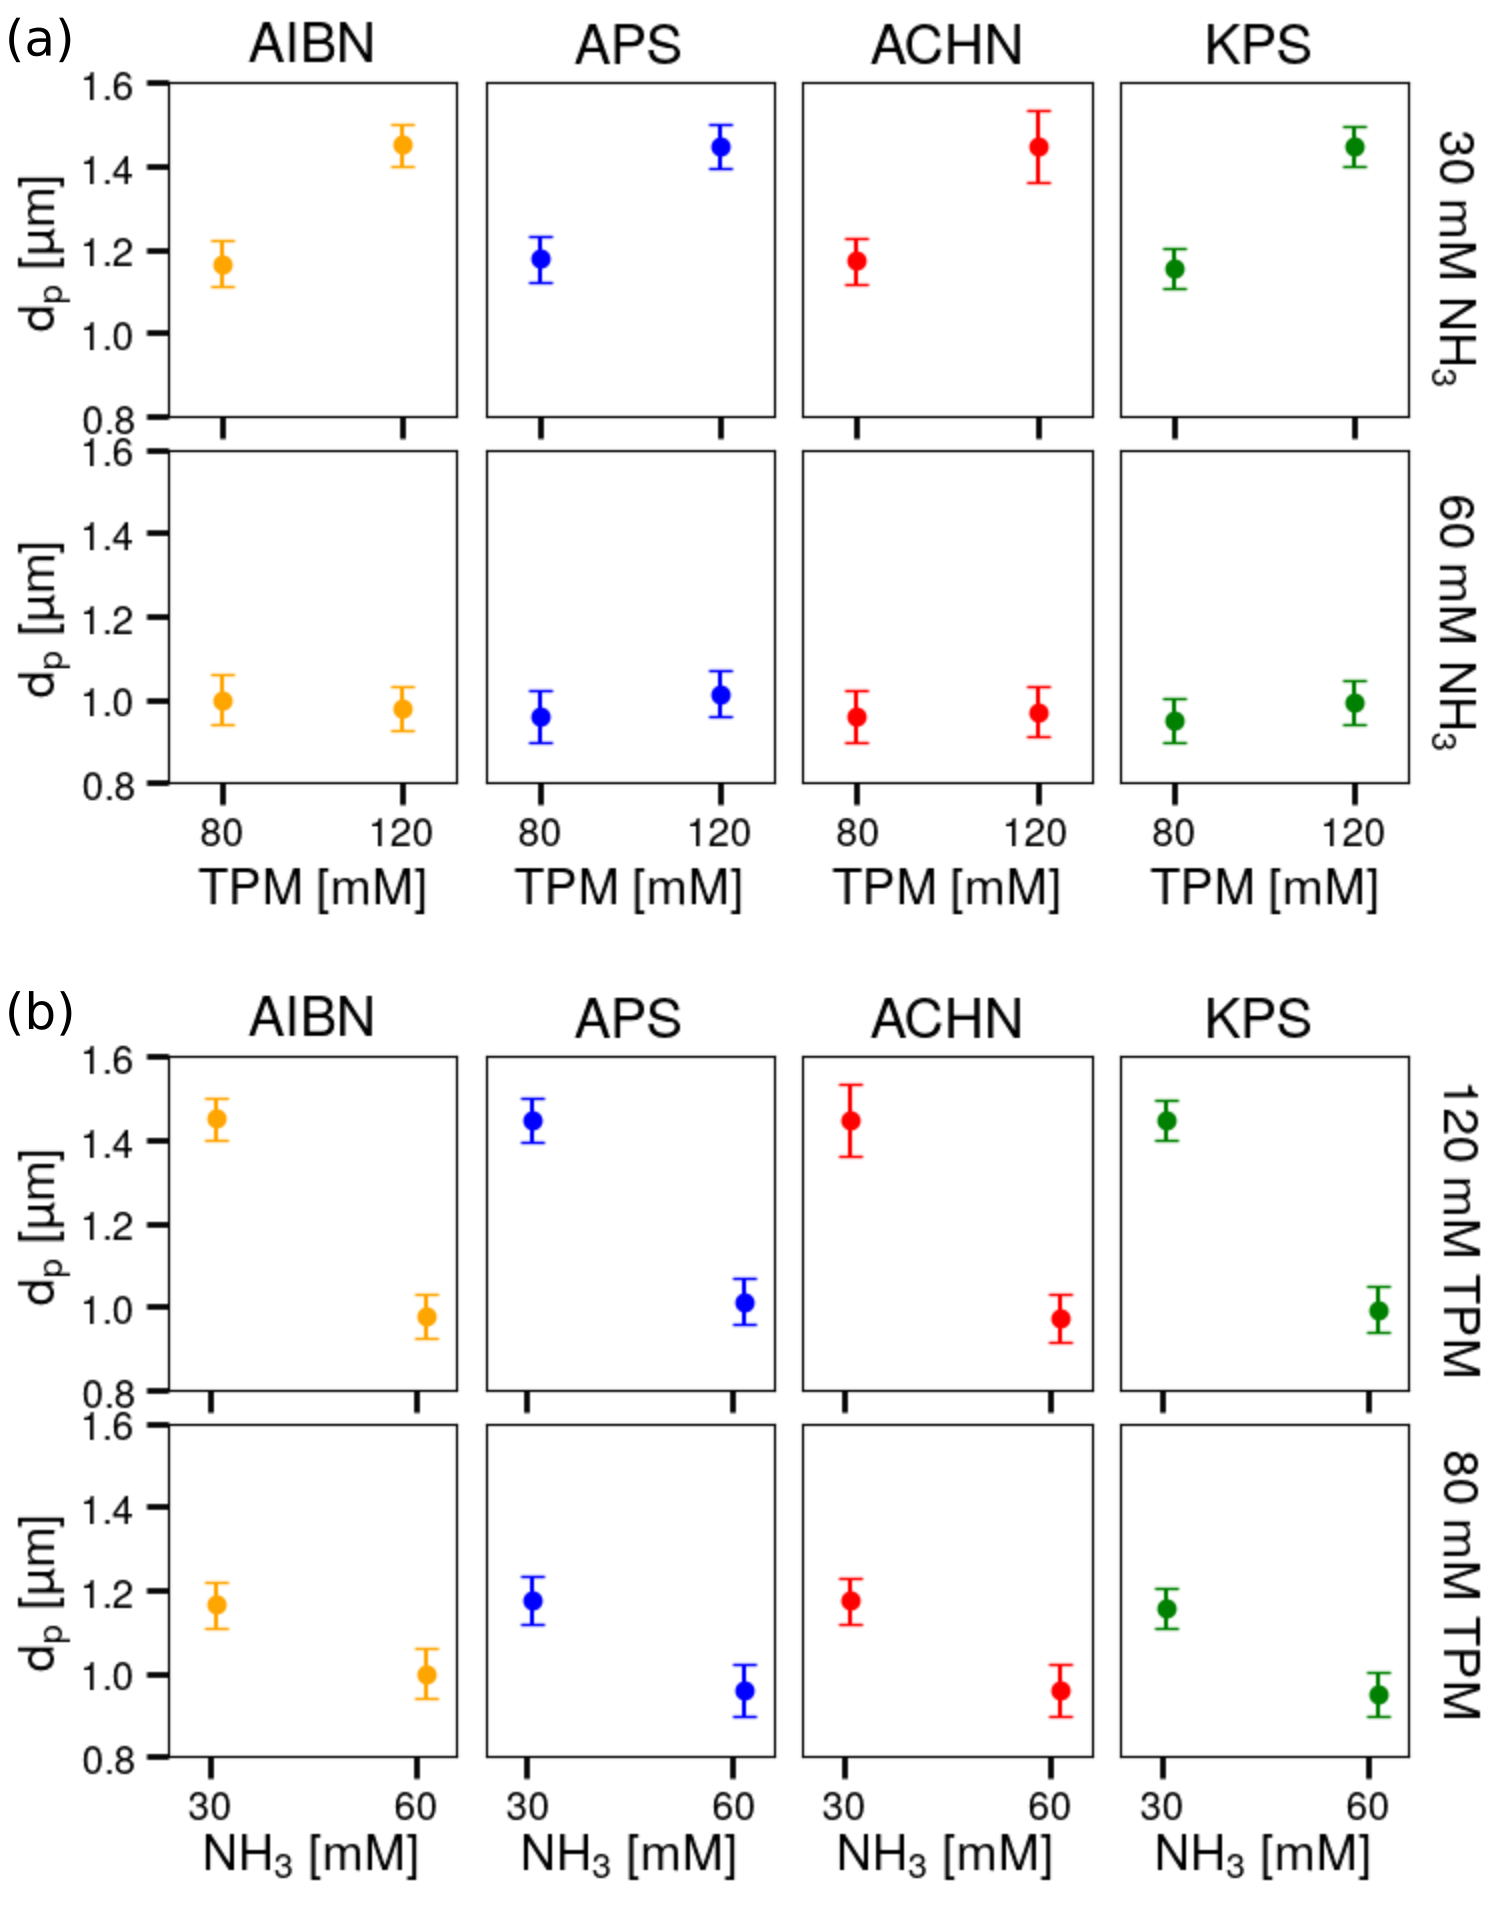
\includegraphics[width=0.5\textwidth]{longitudinal_summary_02}
  \caption{
    (a) Median diameter as a function of TPM content
    at fixed ammonia concentration.
    (b) Median diameter as a function of ammonia
    concentration at fixed TPM content.}
  \label{fig:choices}
\end{figure}

Figure~\ref{fig:choices} presents
characterization data from all \num{16} data sets plotted to highlight different
binary choices.
Each point represents the median properties of
one of the samples and is amassed 
from several thousand
individual holographic characterization measurements.
Figure~\ref{fig:choices}(a) 
emphasizes the influence of TPM concentration
on the polymerized particle diameter
for fixed concentration of 
ammonia and choice 
of initiator.
Increasing TPM content increases particle
diameter at low concentration of ammonia,
but has less influence at higher concentration
of ammonia.
Increasing the concentration of 
ammonia
therefore improves reproducibility by 
reducing sensitivity to variations in TPM concentration.

Figure~\ref{fig:choices}(b) shows the complementary projection
of the data that emphasizes the influence of
ammonia concentration. 
All eight assays convey the same message:
increasing ammonia concentration
decreases the average particle diameter\DIFdelbegin \DIFdel{.
Increased ammonia }\DIFdelend \DIFaddbegin \DIFadd{, presumably because
increasing pH }\DIFaddend increases surface charge \DIFdelbegin \DIFdel{, 
which promotes nucleated particle stability \mbox{%DIFAUXCMD
\cite{vanderwel17}}\hspace{0pt}%DIFAUXCMD
}\DIFdelend \DIFaddbegin \DIFadd{and so
promotes stability of nucleated particles \mbox{%DIFAUXCMD
\cite{vanderwel17,yeung2003shear}}\hspace{0pt}%DIFAUXCMD
}\DIFaddend . 
This, in turn, favors higher particle number density 
and smaller particle size for a given amount of TPM monomer.
Increasing the number and stability of nuclei 
has the additional effect of improving predictability
of the particle radius by reducing sensitivity to the amount
of TPM.

Choice of initiator has no appreciable 
influence on the \DIFdelbegin \DIFdel{finished }\DIFdelend \DIFaddbegin \DIFadd{polymerized }\DIFaddend particles'
average diameter.
Size selection is predominantly 
determined by nucleation and growth of
oligomerized TPM droplets.
The concentration of ammonia increases the pH and
therefore increases the rate at which TPM hydrolizes and oligomerizes.
Faster nucleation
presumably yields more droplets and reduces the average particle size.
At low concentrations of ammonia, 
oligomerization proceeds more slowly
and \DIFdelbegin \DIFdel{and yields fewer }\DIFdelend \DIFaddbegin \DIFadd{yields fewer of the }\DIFaddend larger droplets.

\begin{figure}
    \centering
    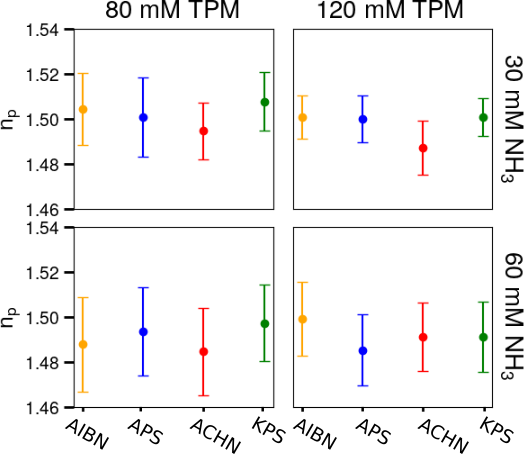
\includegraphics[width=0.5\textwidth]{longitudinal_np_02}
    \caption{Median refractive index reported for each radical initiator
    at fixed concentration of TPM.}
    \label{fig:longitudinal_np}
\end{figure}

The choice of initiator also has no substantial
influence on the particles' refractive indexes,
as shown in Fig.~\ref{fig:longitudinal_np}.
This is surprising because
larger TPM droplets are known to form dimples when polymerized
with the water-soluble initiators \cite{sacanna11}.
Dimpling is believed to result from
surface hardening followed by
ejection of low-molecular-weight oligomers \cite{sacanna11}.
Smaller TPM spheres polymerized with these
initiators do not form dimples \DIFaddbegin \DIFadd{\mbox{%DIFAUXCMD
\cite{vanderwel17}
}\hspace{0pt}%DIFAUXCMD
}\DIFaddend and so might 
be expected to have nonuniform densities
with possible signatures in the measured refractive
index.  In fact, no significant differences are observed.

\section{Summary and Conclusions}
\label{sec:discussion}

We have demonstrated some of the ways in which 
holographic particle characterization
can be used to guide the development of synthesis
protocols for colloidal particles.
Our specific study of monodisperse TPM spheres
examines the influence of particular protocol
choices on the size and refractive index of 
the resulting polymerized spheres. Specifically,
we investigate the roles of stirring rate, 
incubation time, stoichiometry, and choice of
free radical initiator.

Increasing stirring rate is found to increase particle
size at the cost of increasing polydispersity.
Increasing pH through the concentration of ammonia 
decreases particle size and enhances 
reproducibility.

Unlike orthogonal techniques, holographic characterization requires minimal
sample preparation and provides results in minutes,
and so can be used for feedback at all stages in
the synthesis.
Periodically sampling the reaction vessel, for example, 
is useful for determining when droplet growth has
run to completion.

These results demonstrate that holographic characterization can be a valuable
addition to the arsenal of techniques used to design and control colloidal
synthesis protocols.

%DIF < %%%%%%%%%%%%%%%%%%%%%%%%%%%%%%%%%%%%%%%%%%%%%%%%%%%%%%%%%%%%%%%%%%%%
%DIF < % The "Acknowledgement" section can be given in all manuscript
%DIF < % classes.  This should be given within the "acknowledgement"
%DIF < % environment, which will make the correct section or running title.
%DIF < %%%%%%%%%%%%%%%%%%%%%%%%%%%%%%%%%%%%%%%%%%%%%%%%%%%%%%%%%%%%%%%%%%%%
\begin{acknowledgement}
\DIFdelbegin %DIFDELCMD < 

%DIFDELCMD < %%%
\DIFdelend This work was supported primarily by the MRSEC program of
the National Science Foundation through Award Number DMR-1420073.
Additional support was provided by the SBIR program of the
National Science Foundation through Award Number IPP-1519057, and in part by
NASA under \DIFdelbegin \DIFdel{grant award }\DIFdelend \DIFaddbegin \DIFadd{Award Number }\DIFaddend NNX13AR67G.
The Spheryx xSight holographic characterization instrument
used in this study was acquired by the NYU MRSEC as a shared
instrument.
The Zeiss scanning electron microscope used in this study
was acquired under
NSF Award Number DMR-0923251 and is maintained as a shared
facility by the NYU MRSEC.

\end{acknowledgement}

%%%%%%%%%%%%%%%%%%%%%%%%%%%%%%%%%%%%%%%%%%%%%%%%%%%%%%%%%%%%%%%%%%%%%
%% The same is true for Supporting Information, which should use the
%% suppinfo environment.
%%%%%%%%%%%%%%%%%%%%%%%%%%%%%%%%%%%%%%%%%%%%%%%%%%%%%%%%%%%%%%%%%%%%%
%\begin{suppinfo}
%
%None
%
%\end{suppinfo}

%DIF < %%%%%%%%%%%%%%%%%%%%%%%%%%%%%%%%%%%%%%%%%%%%%%%%%%%%%%%%%%%%%%%%%%%%
%DIF < % The appropriate \bibliography command should be placed here.
%DIF < % Notice that the class file automatically sets \bibliographystyle
%DIF < % and also names the section correctly.
%DIF < %%%%%%%%%%%%%%%%%%%%%%%%%%%%%%%%%%%%%%%%%%%%%%%%%%%%%%%%%%%%%%%%%%%%
%DIF <  \bibliography{synthesis}
\DIFdelbegin %DIFDELCMD < \providecommand{\latin}[1]{#1}
%DIFDELCMD < \makeatletter
%DIFDELCMD < \providecommand{\doi}
%DIFDELCMD <   {\begingroup\let\do\@makeother\dospecials
%DIFDELCMD <   \catcode%%%
\DIFdel{`\{=1 }%DIFDELCMD < \catcode%%%
\DIFdel{`\}=2 }%DIFDELCMD < \doi@aux}
%DIFDELCMD < \providecommand{\doi@aux}[1]{\endgroup\texttt{#1}}
%DIFDELCMD < \makeatother
%DIFDELCMD < \providecommand*\mcitethebibliography{\thebibliography}
%DIFDELCMD < \csname %%%
\DIFdel{@ifundefined}%DIFDELCMD < \endcsname{endmcitethebibliography}
%DIFDELCMD <   {\let\endmcitethebibliography\endthebibliography}{}
%DIFDELCMD < \begin{mcitethebibliography}{29}
%DIFDELCMD < \providecommand*\natexlab[1]{#1}
%DIFDELCMD < \providecommand*\mciteSetBstSublistMode[1]{}
%DIFDELCMD < \providecommand*\mciteSetBstMaxWidthForm[2]{}
%DIFDELCMD < \providecommand*\mciteBstWouldAddEndPuncttrue
%DIFDELCMD <   {\def\EndOfBibitem{\unskip.}}
%DIFDELCMD < \providecommand*\mciteBstWouldAddEndPunctfalse
%DIFDELCMD <   {\let\EndOfBibitem\relax}
%DIFDELCMD < \providecommand*\mciteSetBstMidEndSepPunct[3]{}
%DIFDELCMD < \providecommand*\mciteSetBstSublistLabelBeginEnd[3]{}
%DIFDELCMD < \providecommand*\EndOfBibitem{}
%DIFDELCMD < \mciteSetBstSublistMode{f}
%DIFDELCMD < \mciteSetBstMaxWidthForm{subitem}{(\alph{mcitesubitemcount})}
%DIFDELCMD < \mciteSetBstSublistLabelBeginEnd
%DIFDELCMD <   {\mcitemaxwidthsubitemform\space}
%DIFDELCMD <   {\relax}
%DIFDELCMD <   {\relax}
%DIFDELCMD < 

%DIFDELCMD < \bibitem[Backus and Williams(1949)Backus, and Williams]{backus1949small}
%DIFDELCMD < %%%
\DIFdel{Backus,~R.~C.; Williams,~R.~C. Small spherical particles of exceptionally
  uniform size. }\emph{\DIFdel{J. Appl. Phys.}} %DIFAUXCMD
\textbf{\DIFdel{1949}}%DIFAUXCMD
\DIFdel{, }\emph{\DIFdel{20}}%DIFAUXCMD
\DIFdel{, 224--225}%DIFDELCMD < \relax
%DIFDELCMD < \mciteBstWouldAddEndPuncttrue
%DIFDELCMD < \mciteSetBstMidEndSepPunct{\mcitedefaultmidpunct}
%DIFDELCMD < {\mcitedefaultendpunct}{\mcitedefaultseppunct}\relax
%DIFDELCMD < \EndOfBibitem
%DIFDELCMD < \bibitem[Gerould(1950)]{gerould1950comments}
%DIFDELCMD < %%%
\DIFdel{Gerould,~C.~H. Comments on the use of latex spheres as size standards in
  electron microscopy. }\emph{\DIFdel{J. Appl. Phys.}} %DIFAUXCMD
\textbf{\DIFdel{1950}}%DIFAUXCMD
\DIFdel{, }\emph{\DIFdel{21}}%DIFAUXCMD
\DIFdel{,
  183--184}%DIFDELCMD < \relax
%DIFDELCMD < \mciteBstWouldAddEndPuncttrue
%DIFDELCMD < \mciteSetBstMidEndSepPunct{\mcitedefaultmidpunct}
%DIFDELCMD < {\mcitedefaultendpunct}{\mcitedefaultseppunct}\relax
%DIFDELCMD < \EndOfBibitem
%DIFDELCMD < \bibitem[Vanderhoff \latin{et~al.}(1956)Vanderhoff, Vitkuske, Bradford, and
%DIFDELCMD <   Alfrey~Jr]{vanderhoff1956some}
%DIFDELCMD < %%%
\DIFdel{Vanderhoff,~J.; Vitkuske,~J.; Bradford,~E.; Alfrey~Jr,~T. Some factors involved
  in the preparation of uniform particle size latexes. }\emph{\DIFdel{J. Polym. Sci.}}
  %DIFAUXCMD
\textbf{\DIFdel{1956}}%DIFAUXCMD
\DIFdel{, }\emph{\DIFdel{20}}%DIFAUXCMD
\DIFdel{, 225--234}%DIFDELCMD < \relax
%DIFDELCMD < \mciteBstWouldAddEndPuncttrue
%DIFDELCMD < \mciteSetBstMidEndSepPunct{\mcitedefaultmidpunct}
%DIFDELCMD < {\mcitedefaultendpunct}{\mcitedefaultseppunct}\relax
%DIFDELCMD < \EndOfBibitem
%DIFDELCMD < \bibitem[St{\"o}ber \latin{et~al.}(1968)St{\"o}ber, Fink, and
%DIFDELCMD <   Bohn]{stober1968controlled}
%DIFDELCMD < %%%
\DIFdel{St}%DIFDELCMD < {%%%
\DIFdel{\"o}%DIFDELCMD < }%%%
\DIFdel{ber,~W.; Fink,~A.; Bohn,~E. Controlled growth of monodisperse silica
  spheres in the micron size range. }\emph{\DIFdel{J. Colloid Interf. Sci.}}
  %DIFAUXCMD
\textbf{\DIFdel{1968}}%DIFAUXCMD
\DIFdel{, }\emph{\DIFdel{26}}%DIFAUXCMD
\DIFdel{, 62--69}%DIFDELCMD < \relax
%DIFDELCMD < \mciteBstWouldAddEndPuncttrue
%DIFDELCMD < \mciteSetBstMidEndSepPunct{\mcitedefaultmidpunct}
%DIFDELCMD < {\mcitedefaultendpunct}{\mcitedefaultseppunct}\relax
%DIFDELCMD < \EndOfBibitem
%DIFDELCMD < \bibitem[Kotera \latin{et~al.}(1970)Kotera, Furusawa, and
%DIFDELCMD <   Kud{\=o}]{kotera1970colloid}
%DIFDELCMD < %%%
\DIFdel{Kotera,~A.; Furusawa,~K.; Kud}%DIFDELCMD < {%%%
\DIFdel{\=o}%DIFDELCMD < }%%%
\DIFdel{,~K. Colloid chemical studies of polystyrene
  latices polymerized without any surface-active agents. }%DIFDELCMD < {%%%
\DIFdel{I.}%DIFDELCMD < } %%%
\DIFdel{Method for
  preparing monodisperse latices and their characterization. }\emph{\DIFdel{Kolloid Z.
  Z. Polym.}} %DIFAUXCMD
\textbf{\DIFdel{1970}}%DIFAUXCMD
\DIFdel{, }\emph{\DIFdel{240}}%DIFAUXCMD
\DIFdel{, 837--842}%DIFDELCMD < \relax
%DIFDELCMD < \mciteBstWouldAddEndPuncttrue
%DIFDELCMD < \mciteSetBstMidEndSepPunct{\mcitedefaultmidpunct}
%DIFDELCMD < {\mcitedefaultendpunct}{\mcitedefaultseppunct}\relax
%DIFDELCMD < \EndOfBibitem
%DIFDELCMD < \bibitem[De\v{z}eli\'{c} \latin{et~al.}(1970)De\v{z}eli\'{c}, Peters, and
%DIFDELCMD <   De\v{z}eli\'{c}]{dezelic1970preparation}
%DIFDELCMD < %%%
\DIFdel{De\v{z}eli\'{c},~N.; Peters,~J.~J.; De\v{z}eli\'{c},~}%DIFDELCMD < {\relax %%%
\DIFdel{Gj}%DIFDELCMD < }%%%
\DIFdel{. Preparation
  of monodisperse polystyrene latices. }\emph{\DIFdel{Kolloid Z. Z. Polym.}}
  %DIFAUXCMD
\textbf{\DIFdel{1970}}%DIFAUXCMD
\DIFdel{, }\emph{\DIFdel{242}}%DIFAUXCMD
\DIFdel{, 1142--1150}%DIFDELCMD < \relax
%DIFDELCMD < \mciteBstWouldAddEndPuncttrue
%DIFDELCMD < \mciteSetBstMidEndSepPunct{\mcitedefaultmidpunct}
%DIFDELCMD < {\mcitedefaultendpunct}{\mcitedefaultseppunct}\relax
%DIFDELCMD < \EndOfBibitem
%DIFDELCMD < \bibitem[Goodwin \latin{et~al.}(1974)Goodwin, Hearn, Ho, and
%DIFDELCMD <   Ottewill]{goodwin1974studies}
%DIFDELCMD < %%%
\DIFdel{Goodwin,~J.; Hearn,~J.; Ho,~C.; Ottewill,~R. Studies on the preparation and
  characterisation of monodisperse polystyrene latices. }%DIFDELCMD < {%%%
\DIFdel{III.}%DIFDELCMD < } %%%
\DIFdel{Preparation
  without added surface active agents. }\emph{\DIFdel{Colloid Polym. Sci.}}
  %DIFAUXCMD
\textbf{\DIFdel{1974}}%DIFAUXCMD
\DIFdel{, }\emph{\DIFdel{252}}%DIFAUXCMD
\DIFdel{, 464--471}%DIFDELCMD < \relax
%DIFDELCMD < \mciteBstWouldAddEndPuncttrue
%DIFDELCMD < \mciteSetBstMidEndSepPunct{\mcitedefaultmidpunct}
%DIFDELCMD < {\mcitedefaultendpunct}{\mcitedefaultseppunct}\relax
%DIFDELCMD < \EndOfBibitem
%DIFDELCMD < \bibitem[Antl \latin{et~al.}(1986)Antl, Goodwin, Hill, Ottewill, Owens,
%DIFDELCMD <   Papworth, and Waters]{antl1986preparation}
%DIFDELCMD < %%%
\DIFdel{Antl,~L.; Goodwin,~J.; Hill,~R.; Ottewill,~R.~H.; Owens,~S.; Papworth,~S.;
  Waters,~J. The preparation of poly (methyl methacrylate) latices in
  non-aqueous media. }\emph{\DIFdel{Colloids Surf.}} %DIFAUXCMD
\textbf{\DIFdel{1986}}%DIFAUXCMD
\DIFdel{, }\emph{\DIFdel{17}}%DIFAUXCMD
\DIFdel{,
  67--78}%DIFDELCMD < \relax
%DIFDELCMD < \mciteBstWouldAddEndPuncttrue
%DIFDELCMD < \mciteSetBstMidEndSepPunct{\mcitedefaultmidpunct}
%DIFDELCMD < {\mcitedefaultendpunct}{\mcitedefaultseppunct}\relax
%DIFDELCMD < \EndOfBibitem
%DIFDELCMD < \bibitem[Yamada \latin{et~al.}(1985)Yamada, Miyamoto, and Koizumi]{yamada85}
%DIFDELCMD < %%%
\DIFdel{Yamada,~Y.; Miyamoto,~K.; Koizumi,~A. Size determination of latex particles by
  electron microscopy. }\emph{\DIFdel{Aerosol Sci. Techn.}} %DIFAUXCMD
\textbf{\DIFdel{1985}}%DIFAUXCMD
\DIFdel{, }\emph{\DIFdel{4}}%DIFAUXCMD
\DIFdel{,
  227--232}%DIFDELCMD < \relax
%DIFDELCMD < \mciteBstWouldAddEndPuncttrue
%DIFDELCMD < \mciteSetBstMidEndSepPunct{\mcitedefaultmidpunct}
%DIFDELCMD < {\mcitedefaultendpunct}{\mcitedefaultseppunct}\relax
%DIFDELCMD < \EndOfBibitem
%DIFDELCMD < \bibitem[Giesche(2006)]{giesche2006mercury}
%DIFDELCMD < %%%
\DIFdel{Giesche,~H. Mercury porosimetry: a general (practical) overview. }\emph{\DIFdel{Part.
  Part. Syst. Character.}} %DIFAUXCMD
\textbf{\DIFdel{2006}}%DIFAUXCMD
\DIFdel{, }\emph{\DIFdel{23}}%DIFAUXCMD
\DIFdel{, 9--19}%DIFDELCMD < \relax
%DIFDELCMD < \mciteBstWouldAddEndPuncttrue
%DIFDELCMD < \mciteSetBstMidEndSepPunct{\mcitedefaultmidpunct}
%DIFDELCMD < {\mcitedefaultendpunct}{\mcitedefaultseppunct}\relax
%DIFDELCMD < \EndOfBibitem
%DIFDELCMD < \bibitem[Rouquerol \latin{et~al.}(1994)Rouquerol, Avnir, Fairbridge, Everett,
%DIFDELCMD <   Haynes, Pernicone, Ramsay, Sing, and Unger]{rouquerol1994}
%DIFDELCMD < %%%
\DIFdel{Rouquerol,~J.; Avnir,~D.; Fairbridge,~C.; Everett,~D.; Haynes,~J.;
  Pernicone,~N.; Ramsay,~J.; Sing,~K.; Unger,~K. Recommendations for the
  characterization of porous solids (Technical Report). }\emph{\DIFdel{Pure Appl. Chem.}}
  %DIFAUXCMD
\textbf{\DIFdel{1994}}%DIFAUXCMD
\DIFdel{, }\emph{\DIFdel{66}}%DIFAUXCMD
\DIFdel{, 1739--1758}%DIFDELCMD < \relax
%DIFDELCMD < \mciteBstWouldAddEndPuncttrue
%DIFDELCMD < \mciteSetBstMidEndSepPunct{\mcitedefaultmidpunct}
%DIFDELCMD < {\mcitedefaultendpunct}{\mcitedefaultseppunct}\relax
%DIFDELCMD < \EndOfBibitem
%DIFDELCMD < \bibitem[Chou and Kerker(1956)Chou, and Kerker]{chou54}
%DIFDELCMD < %%%
\DIFdel{Chou,~A.; Kerker,~M. The refractive index of colloidal sols. }\emph{\DIFdel{J. Phys.
  Chem.}} %DIFAUXCMD
\textbf{\DIFdel{1956}}%DIFAUXCMD
\DIFdel{, }\emph{\DIFdel{60}}%DIFAUXCMD
\DIFdel{, 562--564}%DIFDELCMD < \relax
%DIFDELCMD < \mciteBstWouldAddEndPuncttrue
%DIFDELCMD < \mciteSetBstMidEndSepPunct{\mcitedefaultmidpunct}
%DIFDELCMD < {\mcitedefaultendpunct}{\mcitedefaultseppunct}\relax
%DIFDELCMD < \EndOfBibitem
%DIFDELCMD < \bibitem[van~der Wel \latin{et~al.}(2017)van~der Wel, Bhan, Verweij, Frijters,
%DIFDELCMD <   Gong, Hollingsworth, Sacanna, and Kraft]{vanderwel17}
%DIFDELCMD < %%%
\DIFdel{van~der Wel,~C.; Bhan,~R.~K.; Verweij,~R.~W.; Frijters,~H.~C.; Gong,~Z.;
  Hollingsworth,~A.~D.; Sacanna,~S.; Kraft,~D.~J. Preparation of colloidal
  organosilica spheres through spontaneous emulsification. }\emph{\DIFdel{Langmuir}}
  %DIFAUXCMD
\textbf{\DIFdel{2017}}%DIFAUXCMD
\DIFdel{, }\emph{\DIFdel{33}}%DIFAUXCMD
\DIFdel{, 8174--8180}%DIFDELCMD < \relax
%DIFDELCMD < \mciteBstWouldAddEndPuncttrue
%DIFDELCMD < \mciteSetBstMidEndSepPunct{\mcitedefaultmidpunct}
%DIFDELCMD < {\mcitedefaultendpunct}{\mcitedefaultseppunct}\relax
%DIFDELCMD < \EndOfBibitem
%DIFDELCMD < \bibitem[Sacanna \latin{et~al.}(2011)Sacanna, Irvine, Rossi, and
%DIFDELCMD <   Pine]{sacanna11}
%DIFDELCMD < %%%
\DIFdel{Sacanna,~S.; Irvine,~W. T.~M.; Rossi,~L.; Pine,~D.~J. Lock and key colloids
  through polymerization-induced buckling of monodisperse silicon oil droplets.
  }\emph{\DIFdel{Soft Matter}} %DIFAUXCMD
\textbf{\DIFdel{2011}}%DIFAUXCMD
\DIFdel{, }\emph{\DIFdel{7}}%DIFAUXCMD
\DIFdel{, 1631--1634}%DIFDELCMD < \relax
%DIFDELCMD < \mciteBstWouldAddEndPuncttrue
%DIFDELCMD < \mciteSetBstMidEndSepPunct{\mcitedefaultmidpunct}
%DIFDELCMD < {\mcitedefaultendpunct}{\mcitedefaultseppunct}\relax
%DIFDELCMD < \EndOfBibitem
%DIFDELCMD < \bibitem[Liu \latin{et~al.}(2016)Liu, Edmond, Curran, Bryant, Peng, Aarts,
%DIFDELCMD <   Sacanna, and Dullens]{liu16}
%DIFDELCMD < %%%
\DIFdel{Liu,~Y.; Edmond,~K.~V.; Curran,~A.; Bryant,~C.; Peng,~B.; Aarts,~D. G. A.~L.;
  Sacanna,~S.; Dullens,~R. P.~A. Core–shell particles for simultaneous 3D
  imaging and optical tweezing in dense colloidal materials. }\emph{\DIFdel{Adv. Mater.}}
  %DIFAUXCMD
\textbf{\DIFdel{2016}}%DIFAUXCMD
\DIFdel{, }\emph{\DIFdel{28}}%DIFAUXCMD
\DIFdel{, 8001--8006}%DIFDELCMD < \relax
%DIFDELCMD < \mciteBstWouldAddEndPuncttrue
%DIFDELCMD < \mciteSetBstMidEndSepPunct{\mcitedefaultmidpunct}
%DIFDELCMD < {\mcitedefaultendpunct}{\mcitedefaultseppunct}\relax
%DIFDELCMD < \EndOfBibitem
%DIFDELCMD < \bibitem[van~der Wel \latin{et~al.}(2018)van~der Wel, van~de Stolpe, Verweij,
%DIFDELCMD <   and Kraft]{vanderwel18}
%DIFDELCMD < %%%
\DIFdel{van~der Wel,~C.; van~de Stolpe,~G.~L.; Verweij,~R.~W.; Kraft,~D.~J.
  Micrometer-sized TPM emulsion droplets with surface-mobile binding groups.
  }\emph{\DIFdel{J. Phys. Cond. Matt.}} %DIFAUXCMD
\textbf{\DIFdel{2018}}%DIFAUXCMD
\DIFdel{, }\emph{\DIFdel{30}}%DIFAUXCMD
\DIFdel{, 094005}%DIFDELCMD < \relax
%DIFDELCMD < \mciteBstWouldAddEndPuncttrue
%DIFDELCMD < \mciteSetBstMidEndSepPunct{\mcitedefaultmidpunct}
%DIFDELCMD < {\mcitedefaultendpunct}{\mcitedefaultseppunct}\relax
%DIFDELCMD < \EndOfBibitem
%DIFDELCMD < \bibitem[Lee \latin{et~al.}(2007)Lee, Roichman, Yi, Kim, Yang, van Blaaderen,
%DIFDELCMD <   van Oostrum, and Grier]{lee07a}
%DIFDELCMD < %%%
\DIFdel{Lee,~S.-H.; Roichman,~Y.; Yi,~G.-R.; Kim,~S.-H.; Yang,~S.-M.; van
  Blaaderen,~A.; van Oostrum,~P.; Grier,~D.~G. Characterizing and tracking
  single colloidal particles with video holographic microscopy. }\emph{\DIFdel{Opt.
  Express}} %DIFAUXCMD
\textbf{\DIFdel{2007}}%DIFAUXCMD
\DIFdel{, }\emph{\DIFdel{15}}%DIFAUXCMD
\DIFdel{, 18275--18282}%DIFDELCMD < \relax
%DIFDELCMD < \mciteBstWouldAddEndPuncttrue
%DIFDELCMD < \mciteSetBstMidEndSepPunct{\mcitedefaultmidpunct}
%DIFDELCMD < {\mcitedefaultendpunct}{\mcitedefaultseppunct}\relax
%DIFDELCMD < \EndOfBibitem
%DIFDELCMD < \bibitem[Cheong \latin{et~al.}(2010)Cheong, Krishnatreya, and Grier]{cheong10a}
%DIFDELCMD < %%%
\DIFdel{Cheong,~F.~C.; Krishnatreya,~B.~J.; Grier,~D.~G. Strategies for
  three-dimensional particle tracking with holographic video microscopy.
  }\emph{\DIFdel{Opt. Express}} %DIFAUXCMD
\textbf{\DIFdel{2010}}%DIFAUXCMD
\DIFdel{, }\emph{\DIFdel{18}}%DIFAUXCMD
\DIFdel{, 13563--13573}%DIFDELCMD < \relax
%DIFDELCMD < \mciteBstWouldAddEndPuncttrue
%DIFDELCMD < \mciteSetBstMidEndSepPunct{\mcitedefaultmidpunct}
%DIFDELCMD < {\mcitedefaultendpunct}{\mcitedefaultseppunct}\relax
%DIFDELCMD < \EndOfBibitem
%DIFDELCMD < \bibitem[Jung \latin{et~al.}(2002)Jung, Park, Song, O, and Eom]{jung02}
%DIFDELCMD < %%%
\DIFdel{Jung,~K.; Park,~B.; Song,~W.; O,~B.-H.; Eom,~T. Measurement of 100-nm
  polystyrene sphere by transmission electron microscope. }\emph{\DIFdel{Powder Tech.}}
  %DIFAUXCMD
\textbf{\DIFdel{2002}}%DIFAUXCMD
\DIFdel{, }\emph{\DIFdel{126}}%DIFAUXCMD
\DIFdel{, 255--265}%DIFDELCMD < \relax
%DIFDELCMD < \mciteBstWouldAddEndPuncttrue
%DIFDELCMD < \mciteSetBstMidEndSepPunct{\mcitedefaultmidpunct}
%DIFDELCMD < {\mcitedefaultendpunct}{\mcitedefaultseppunct}\relax
%DIFDELCMD < \EndOfBibitem
%DIFDELCMD < \bibitem[Alexander \latin{et~al.}(1981)Alexander, Killey, Meeten, and
%DIFDELCMD <   Senior]{alexander81}
%DIFDELCMD < %%%
\DIFdel{Alexander,~K.; Killey,~A.; Meeten,~G.; Senior,~M. Refractive index of
  concentrated colloidal dispersions. }\emph{\DIFdel{J. Chem. Soc. Faraday Trans. 2}}
  %DIFAUXCMD
\textbf{\DIFdel{1981}}%DIFAUXCMD
\DIFdel{, }\emph{\DIFdel{77}}%DIFAUXCMD
\DIFdel{, 361--372}%DIFDELCMD < \relax
%DIFDELCMD < \mciteBstWouldAddEndPuncttrue
%DIFDELCMD < \mciteSetBstMidEndSepPunct{\mcitedefaultmidpunct}
%DIFDELCMD < {\mcitedefaultendpunct}{\mcitedefaultseppunct}\relax
%DIFDELCMD < \EndOfBibitem
%DIFDELCMD < \bibitem[Hal{\'a}sz \latin{et~al.}(2007)Hal{\'a}sz, Gy{\"u}re, J{\'a}nosi,
%DIFDELCMD <   Szab{\'o}, and T{\'e}l]{halasz2007vortex}
%DIFDELCMD < %%%
\DIFdel{Hal}%DIFDELCMD < {%%%
\DIFdel{\'a}%DIFDELCMD < }%%%
\DIFdel{sz,~G.; Gy}%DIFDELCMD < {%%%
\DIFdel{\"u}%DIFDELCMD < }%%%
\DIFdel{re,~B.; J}%DIFDELCMD < {%%%
\DIFdel{\'a}%DIFDELCMD < }%%%
\DIFdel{nosi,~I.~M.; Szab}%DIFDELCMD < {%%%
\DIFdel{\'o}%DIFDELCMD < }%%%
\DIFdel{,~K.~G.; T}%DIFDELCMD < {%%%
\DIFdel{\'e}%DIFDELCMD < }%%%
\DIFdel{l,~T.
  Vortex flow generated by a magnetic stirrer. }\emph{\DIFdel{Am. J. Phys.}}
  %DIFAUXCMD
\textbf{\DIFdel{2007}}%DIFAUXCMD
\DIFdel{, }\emph{\DIFdel{75}}%DIFAUXCMD
\DIFdel{, 1092--1098}%DIFDELCMD < \relax
%DIFDELCMD < \mciteBstWouldAddEndPuncttrue
%DIFDELCMD < \mciteSetBstMidEndSepPunct{\mcitedefaultmidpunct}
%DIFDELCMD < {\mcitedefaultendpunct}{\mcitedefaultseppunct}\relax
%DIFDELCMD < \EndOfBibitem
%DIFDELCMD < \bibitem[Oles(1992)]{oles1992shear}
%DIFDELCMD < %%%
\DIFdel{Oles,~V. Shear-induced aggregation and breakup of polystyrene latex particles.
  }\emph{\DIFdel{J. Colloid Interface Sci.}} %DIFAUXCMD
\textbf{\DIFdel{1992}}%DIFAUXCMD
\DIFdel{, }\emph{\DIFdel{154}}%DIFAUXCMD
\DIFdel{, 351--358}%DIFDELCMD < \relax
%DIFDELCMD < \mciteBstWouldAddEndPuncttrue
%DIFDELCMD < \mciteSetBstMidEndSepPunct{\mcitedefaultmidpunct}
%DIFDELCMD < {\mcitedefaultendpunct}{\mcitedefaultseppunct}\relax
%DIFDELCMD < \EndOfBibitem
%DIFDELCMD < \bibitem[Eggersdorfer \latin{et~al.}(2010)Eggersdorfer, Kadau, Herrmann, and
%DIFDELCMD <   Pratsinis]{eggersdorfer2010fragmentation}
%DIFDELCMD < %%%
\DIFdel{Eggersdorfer,~M.; Kadau,~D.; Herrmann,~H.~J.; Pratsinis,~S.~E. Fragmentation
  and restructuring of soft-agglomerates under shear. }\emph{\DIFdel{J. Colloid
  Interface Sci.}} %DIFAUXCMD
\textbf{\DIFdel{2010}}%DIFAUXCMD
\DIFdel{, }\emph{\DIFdel{342}}%DIFAUXCMD
\DIFdel{, 261--268}%DIFDELCMD < \relax
%DIFDELCMD < \mciteBstWouldAddEndPuncttrue
%DIFDELCMD < \mciteSetBstMidEndSepPunct{\mcitedefaultmidpunct}
%DIFDELCMD < {\mcitedefaultendpunct}{\mcitedefaultseppunct}\relax
%DIFDELCMD < \EndOfBibitem
%DIFDELCMD < \bibitem[Chern(2006)]{chern06}
%DIFDELCMD < %%%
\DIFdel{Chern,~C. Emulsion polymerization mechanisms and kinetics. }\emph{\DIFdel{Prog. Polym.
  Sci.}} %DIFAUXCMD
\textbf{\DIFdel{2006}}%DIFAUXCMD
\DIFdel{, }\emph{\DIFdel{31}}%DIFAUXCMD
\DIFdel{, 443--486}%DIFDELCMD < \relax
%DIFDELCMD < \mciteBstWouldAddEndPuncttrue
%DIFDELCMD < \mciteSetBstMidEndSepPunct{\mcitedefaultmidpunct}
%DIFDELCMD < {\mcitedefaultendpunct}{\mcitedefaultseppunct}\relax
%DIFDELCMD < \EndOfBibitem
%DIFDELCMD < \bibitem[Arshady(1992)]{arshady92}
%DIFDELCMD < %%%
\DIFdel{Arshady,~R. Suspension, emulsion, and dispersion polymerization: A
  methodological survey. }\emph{\DIFdel{Colloid Polym. Sci.}} %DIFAUXCMD
\textbf{\DIFdel{1992}}%DIFAUXCMD
\DIFdel{, }\emph{\DIFdel{270}}%DIFAUXCMD
\DIFdel{,
  717--732}%DIFDELCMD < \relax
%DIFDELCMD < \mciteBstWouldAddEndPuncttrue
%DIFDELCMD < \mciteSetBstMidEndSepPunct{\mcitedefaultmidpunct}
%DIFDELCMD < {\mcitedefaultendpunct}{\mcitedefaultseppunct}\relax
%DIFDELCMD < \EndOfBibitem
%DIFDELCMD < \bibitem[Mazzoli and Favoni(2012)Mazzoli, and Favoni]{mazzoli12}
%DIFDELCMD < %%%
\DIFdel{Mazzoli,~A.; Favoni,~O. Particle size, size distribution and morphological
  evaluation of airborne dust particles of diverse woods by Scanning Electron
  Microscopy and image processing program. }\emph{\DIFdel{Powder Tech.}} %DIFAUXCMD
\textbf{\DIFdel{2012}}%DIFAUXCMD
\DIFdel{,
  }\emph{\DIFdel{225}}%DIFAUXCMD
\DIFdel{, 65--71}%DIFDELCMD < \relax
%DIFDELCMD < \mciteBstWouldAddEndPuncttrue
%DIFDELCMD < \mciteSetBstMidEndSepPunct{\mcitedefaultmidpunct}
%DIFDELCMD < {\mcitedefaultendpunct}{\mcitedefaultseppunct}\relax
%DIFDELCMD < \EndOfBibitem
%DIFDELCMD < \bibitem[Borisov \latin{et~al.}(2015)Borisov, Luksha, and
%DIFDELCMD <   Rashidova]{borisov2015kinetic}
%DIFDELCMD < %%%
\DIFdel{Borisov,~I.; Luksha,~R.; Rashidova,~S. Kinetic features of ammonium persulfate
  decomposition in aqueous medium. }\emph{\DIFdel{Russian Chem. Bull.}} %DIFAUXCMD
\textbf{\DIFdel{2015}}%DIFAUXCMD
\DIFdel{,
  }\emph{\DIFdel{64}}%DIFAUXCMD
\DIFdel{, 2512--2513}%DIFDELCMD < \relax
%DIFDELCMD < \mciteBstWouldAddEndPuncttrue
%DIFDELCMD < \mciteSetBstMidEndSepPunct{\mcitedefaultmidpunct}
%DIFDELCMD < {\mcitedefaultendpunct}{\mcitedefaultseppunct}\relax
%DIFDELCMD < \EndOfBibitem
%DIFDELCMD < \bibitem[Beylerian \latin{et~al.}(2002)Beylerian, Vardanyan, Harutyunyan, and
%DIFDELCMD <   Vardanyan]{beylerian2002kinetics}
%DIFDELCMD < %%%
\DIFdel{Beylerian,~N.~M.; Vardanyan,~L.~R.; Harutyunyan,~R.~S.; Vardanyan,~R.~L.
  Kinetics and mechanism of potassium persulfate decomposition in aqueous
  solutions studied by a gasometric method. }\emph{\DIFdel{Macromol. Chem. Phys.}}
  %DIFAUXCMD
\textbf{\DIFdel{2002}}%DIFAUXCMD
\DIFdel{, }\emph{\DIFdel{203}}%DIFAUXCMD
\DIFdel{, 212--218}%DIFDELCMD < \relax
%DIFDELCMD < \mciteBstWouldAddEndPuncttrue
%DIFDELCMD < \mciteSetBstMidEndSepPunct{\mcitedefaultmidpunct}
%DIFDELCMD < {\mcitedefaultendpunct}{\mcitedefaultseppunct}\relax
%DIFDELCMD < \EndOfBibitem
%DIFDELCMD < \end{mcitethebibliography}
%DIFDELCMD < %%%
\DIFdelend \DIFaddbegin \bibliography{synthesis}
\DIFaddend 

\end{document}
%%% Local Variables:
%%% mode: latex
%%% TeX-master: t
%%% End:
